%
% This file is part of the GROMACS molecular simulation package.
%
% Copyright (c) 2013,2014,2015,2016, by the GROMACS development team, led by
% Mark Abraham, David van der Spoel, Berk Hess, and Erik Lindahl,
% and including many others, as listed in the AUTHORS file in the
% top-level source directory and at http://www.gromacs.org.
%
% GROMACS is free software; you can redistribute it and/or
% modify it under the terms of the GNU Lesser General Public License
% as published by the Free Software Foundation; either version 2.1
% of the License, or (at your option) any later version.
%
% GROMACS is distributed in the hope that it will be useful,
% but WITHOUT ANY WARRANTY; without even the implied warranty of
% MERCHANTABILITY or FITNESS FOR A PARTICULAR PURPOSE.  See the GNU
% Lesser General Public License for more details.
%
% You should have received a copy of the GNU Lesser General Public
% License along with GROMACS; if not, see
% http://www.gnu.org/licenses, or write to the Free Software Foundation,
% Inc., 51 Franklin Street, Fifth Floor, Boston, MA  02110-1301  USA.
%
% If you want to redistribute modifications to GROMACS, please
% consider that scientific software is very special. Version
% control is crucial - bugs must be traceable. We will be happy to
% consider code for inclusion in the official distribution, but
% derived work must not be called official GROMACS. Details are found
% in the README & COPYING files - if they are missing, get the
% official version at http://www.gromacs.org.
%
% To help us fund GROMACS development, we humbly ask that you cite
% the research papers on the package. Check out http://www.gromacs.org.

\chapter{Special Topics}
\label{ch:special}


\section{Free energy implementation}
\label{sec:dgimplement}
For free energy calculations, there are two things that must be
specified; the end states, and the pathway connecting the end states.
The end states can be specified in two ways.  The most straightforward
is through the specification of end states in the topology file.  Most
potential forms support both an $A$ state and a $B$ state. Whenever both
states are specified, then the $A$ state corresponds to the initial free
energy state, and the $B$ state corresponds to the final state.

In some cases, the end state can also be defined in some cases without
altering the topology, solely through the {\tt .mdp} file, through the use
of the {\tt couple-moltype},{\tt couple-lambda0}, {\tt couple-lambda1}, and
{\tt couple-intramol} mdp keywords.  Any molecule type selected in
{\tt couple-moltype} will automatically have a $B$ state implicitly
constructed (and the $A$ state redefined) according to the {\tt couple-lambda}
keywords. {\tt couple-lambda0} and {\tt couple-lambda1} define the non-bonded
parameters that are present in the $A$ state ({\tt couple-lambda0})
and the $B$ state ({\tt couple-lambda1}).  The choices are 'q','vdw', and
'vdw-q'; these indicate the Coulombic, van der Waals, or both parameters
that are turned on in the respective state.

Once the end states are defined, then the path between the end states
has to be defined. This path is defined solely in the .mdp file.
Starting in 4.6, $\lambda$ is a vector of components, with Coulombic,
van der Waals, bonded, restraint, and mass components all able to be
adjusted independently.  This makes it possible to turn off the
Coulombic term linearly, and then the van der Waals using soft core,
all in the same simulation.  This is especially useful for replica
exchange or expanded ensemble simulations, where it is important to
sample all the way from interacting to non-interacting states in the
same simulation to improve sampling.

{\tt fep-lambdas} is the default array of $\lambda$ values ranging
from 0 to 1.  All of the other lambda arrays use the values in this
array if they are not specified.  The previous behavior, where the
pathway is controlled by a single $\lambda$ variable, can be preserved
by using only {\tt fep-lambdas} to define the pathway.

For example, if you wanted to first to change the Coulombic terms,
then the van der Waals terms, changing bonded at the same time rate as
the van der Waals, but changing the restraints throughout the first
two-thirds of the simulation, then you could use this $\lambda$ vector:

\begin{verbatim}
coul-lambdas           = 0.0 0.2 0.5 1.0 1.0 1.0 1.0 1.0 1.0 1.0
vdw-lambdas            = 0.0 0.0 0.0 0.0 0.4 0.5 0.6 0.7 0.8 1.0
bonded-lambdas         = 0.0 0.0 0.0 0.0 0.4 0.5 0.6 0.7 0.8 1.0
restraint-lambdas      = 0.0 0.0 0.1 0.2 0.3 0.5 0.7 1.0 1.0 1.0
\end{verbatim}

This is also equivalent to:

\begin{verbatim}
fep-lambdas            = 0.0 0.0 0.0 0.0 0.4 0.5 0.6 0.7 0.8 1.0
coul-lambdas           = 0.0 0.2 0.5 1.0 1.0 1.0 1.0 1.0 1.0 1.0
restraint-lambdas      = 0.0 0.0 0.1 0.2 0.3 0.5 0.7 1.0 1.0 1.0
\end{verbatim}
The {\tt fep-lambda array}, in this case, is being used as the default to
fill in the bonded and van der Waals $\lambda$ arrays.  Usually, it's best to fill
in all arrays explicitly, just to make sure things are properly
assigned.

If you want to turn on only restraints going from $A$ to $B$, then it would be:
\begin{verbatim}
restraint-lambdas      = 0.0 0.1 0.2 0.4 0.6 1.0
\end{verbatim}
and all of the other components of the $\lambda$ vector would be left in the $A$ state.

To compute free energies with a vector $\lambda$ using
thermodynamic integration, then the TI equation becomes vector equation:
\beq
\Delta F = \int \langle \nabla H \rangle \cdot d\vec{\lambda}
\eeq
or for finite differences:
\beq
\Delta F \approx \int \sum \langle \nabla H \rangle \cdot \Delta\lambda
\eeq

The external {\tt pymbar} script downloaded from https://SimTK.org/home/pymbar can
compute this integral automatically from the {\gromacs} dhdl.xvg output.

\section{Potential of mean force}

A potential of mean force (PMF) is a potential that is obtained
by integrating the mean force from an ensemble of configurations.
In {\gromacs}, there are several different methods to calculate the mean force.
Each method has its limitations, which are listed below.
\begin{itemize}
\item{\bf pull code:} between the centers of mass of molecules or groups of molecules.
\item{\bf free-energy code with harmonic bonds or constraints:} between single atoms. 
\item{\bf free-energy code with position restraints:} changing the conformation of a relatively immobile group of atoms.
\item{\bf pull code in limited cases:} between groups of atoms that are
part of a larger molecule for which the bonds are constrained with
SHAKE or LINCS. If the pull group if relatively large,
the pull code can be used.
\end{itemize}
The pull and free-energy code a described in more detail
in the following two sections.

\subsubsection{Entropic effects}
When a distance between two atoms or the centers of mass of two groups
is constrained or restrained, there will be a purely entropic contribution
to the PMF due to the rotation of the two groups~\cite{RMNeumann1980a}.
For a system of two non-interacting masses the potential of mean force is:
\beq
V_{pmf}(r) = -(n_c - 1) k_B T \log(r)
\eeq
where $n_c$ is the number of dimensions in which the constraint works
(i.e. $n_c=3$ for a normal constraint and $n_c=1$ when only
the $z$-direction is constrained).
Whether one needs to correct for this contribution depends on what
the PMF should represent. When one wants to pull a substrate
into a protein, this entropic term indeed contributes to the work to
get the substrate into the protein. But when calculating a PMF
between two solutes in a solvent, for the purpose of simulating
without solvent, the entropic contribution should be removed.
{\bf Note} that this term can be significant; when at 300K the distance is halved,
the contribution is 3.5 kJ~mol$^{-1}$.

\section{Non-equilibrium pulling}
When the distance between two groups is changed continuously,
work is applied to the system, which means that the system is no longer
in equilibrium. Although in the limit of very slow pulling
the system is again in equilibrium, for many systems this limit
is not reachable within reasonable computational time.
However, one can use the Jarzynski relation~\cite{Jarzynski1997a}
to obtain the equilibrium free-energy difference $\Delta G$
between two distances from many non-equilibrium simulations:
\begin{equation}
   \Delta G_{AB} = -k_BT \log \left\langle e^{-\beta W_{AB}} \right\rangle_A
   \label{eq:Jarz}
\end{equation}
where $W_{AB}$ is the work performed to force the system along one path
from state A to B, the angular bracket denotes averaging over
a canonical ensemble of the initial state A and $\beta=1/k_B T$.


\section{The pull code}
\index{center-of-mass pulling}
\label{sec:pull}
The pull code applies forces or constraints between the centers
of mass of one or more pairs of groups of atoms.
Each pull reaction coordinate is called a ``coordinate'' and it operates
on usually two, but sometimes more, pull groups. A pull group can be part of one or more pull
coordinates. Furthermore, a coordinate can also operate on a single group
and an absolute reference position in space.
The distance between a pair of groups can be determined
in 1, 2 or 3 dimensions, or can be along a user-defined vector.
The reference distance can be constant or can change linearly with time.
Normally all atoms are weighted by their mass, but an additional
weighting factor can also be used.
\begin{figure}
\centerline{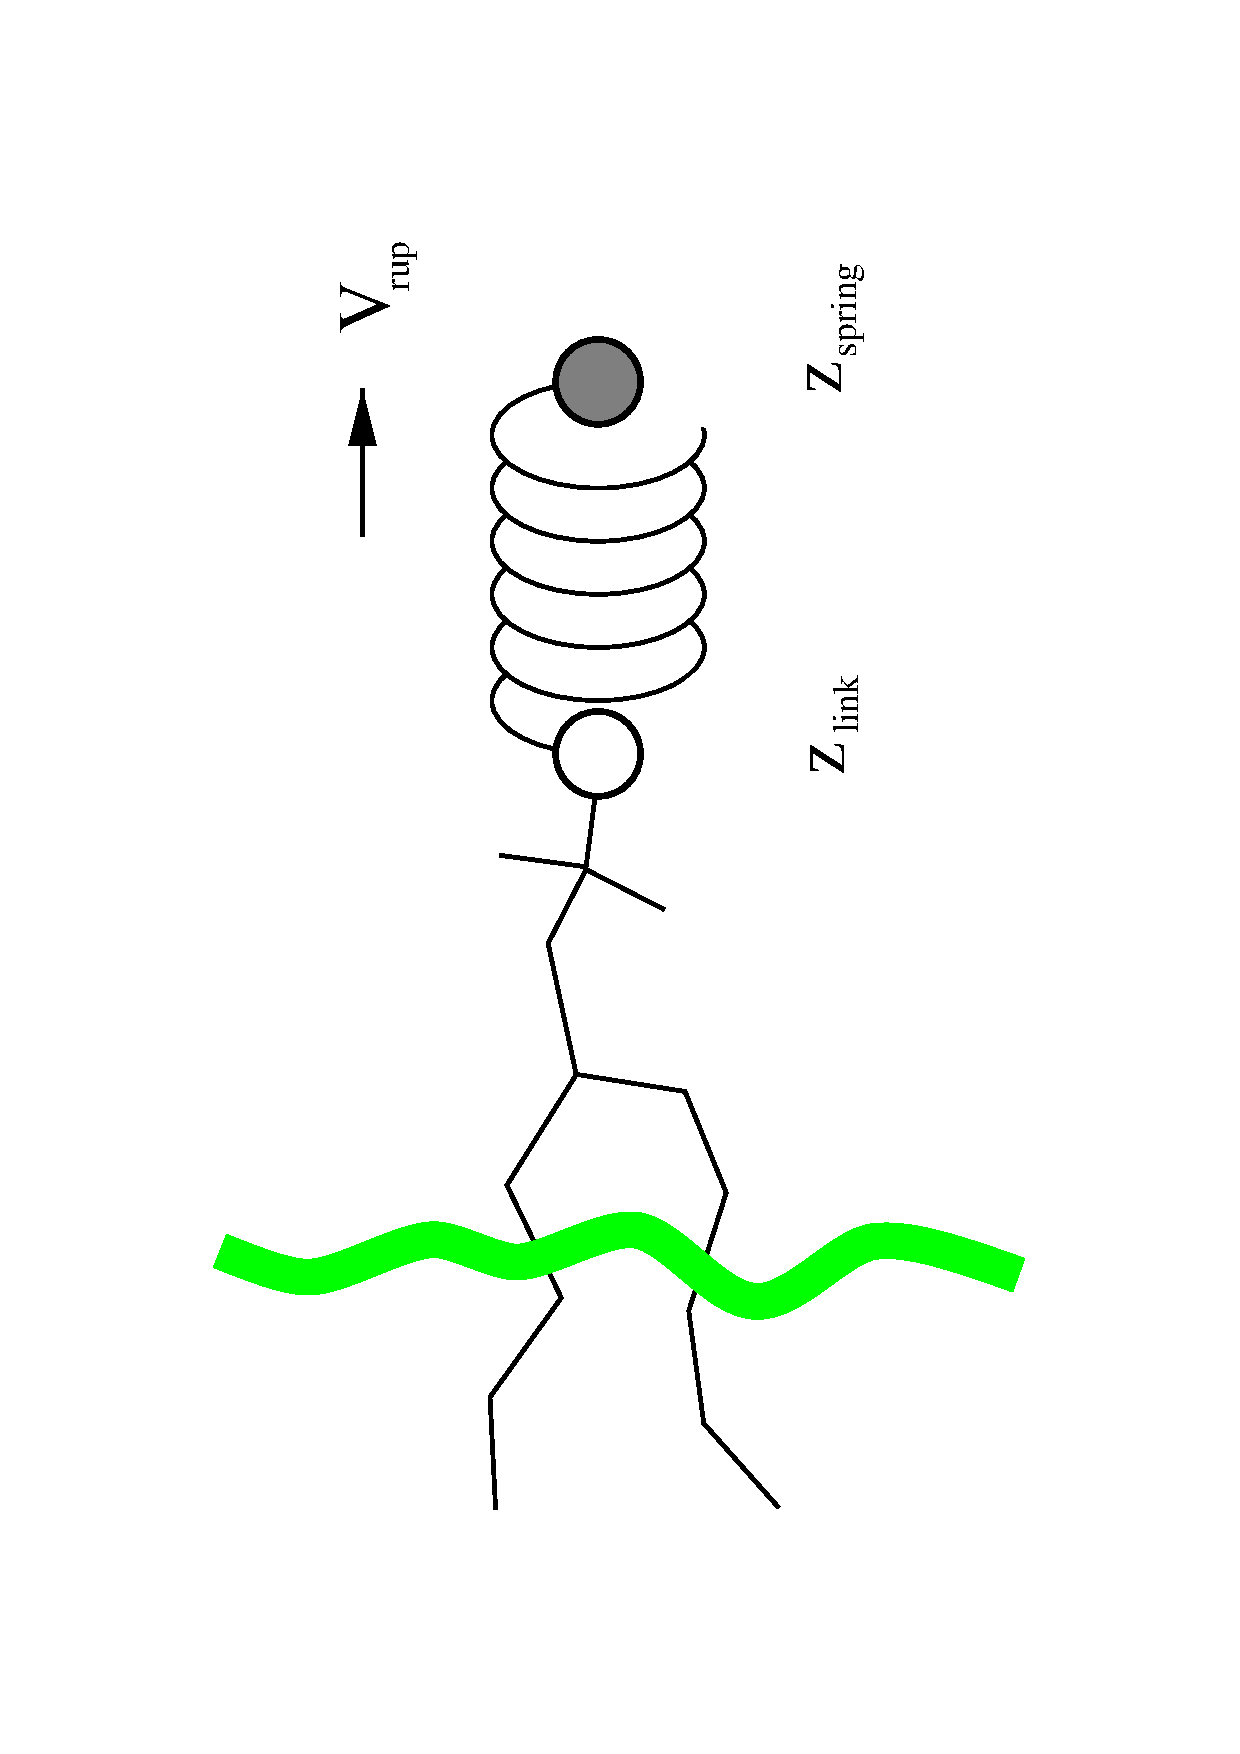
\includegraphics[width=6cm,angle=270]{plots/pull}}
\caption{Schematic picture of pulling a lipid out of a lipid bilayer
with umbrella pulling. $V_{rup}$ is the velocity at which the spring is
retracted, $Z_{link}$ is the atom to which the spring is attached and
$Z_{spring}$ is the location of the spring.}
\label{fig:pull} 
\end{figure}

Several different pull types, i.e. ways to apply the pull force, are supported,
and in all cases the reference distance can be constant
or linearly changing with time.
\begin{enumerate}
\item{\textbf{Umbrella pulling}\swapindexquiet{umbrella}{pulling}}
A harmonic potential is applied between
the centers of mass of two groups.
Thus, the force is proportional to the displacement.
\item{\textbf{Constraint pulling\swapindexquiet{constraint}{pulling}}}
The distance between the centers of mass of two groups is constrained.
The constraint force can be written to a file.
This method uses the SHAKE algorithm but only needs 1 iteration to be
exact if only two groups are constrained. 
\item{\textbf{Constant force pulling}}
A constant force is applied between the centers of mass of two groups.
Thus, the potential is linear.
In this case there is no reference distance of pull rate.
\item{\textbf{Flat bottom pulling}}
Like umbrella pulling, but the potential and force are zero for
coordinate values below ({\tt pull-coord?-type = flat-bottom}) or above
({\tt pull-coord?-type = flat-bottom-high}) a reference value.
This is useful for restraining e.g. the distance
between two molecules to a certain region.
\end{enumerate}
In addition, there are different types of reaction coordinates, so-called pull geometries.
These are set with the {\tt .mdp} option {\tt pull-coord?-geometry}.

\subsubsection{Definition of the center of mass}

In {\gromacs}, there are three ways to define the center of mass of a group.
The standard way is a ``plain'' center of mass, possibly with additional
weighting factors. With periodic boundary conditions it is no longer
possible to uniquely define the center of mass of a group of atoms.
Therefore, a reference atom is used. For determining the center of mass,
for all other atoms in the group, the closest periodic image to the reference
atom is used. This uniquely defines the center of mass.
By default, the middle (determined by the order in the topology) atom
is used as a reference atom, but the user can also select any other atom
if it would be closer to center of the group.

For a layered system, for instance a lipid bilayer, it may be of interest
to calculate the PMF of a lipid as function of its distance
from the whole bilayer. The whole bilayer can be taken as reference
group in that case, but it might also be of interest to define the
reaction coordinate for the PMF more locally. The {\tt .mdp} option
{\tt pull-coord?-geometry = cylinder} does not
use all the atoms of the reference group, but instead dynamically only those
within a cylinder with radius {\tt pull-cylinder-r} around the pull vector going
through the pull group. This only
works for distances defined in one dimension, and the cylinder is
oriented with its long axis along this one dimension. To avoid jumps in
the pull force, contributions of atoms are weighted as a function of distance
(in addition to the mass weighting):
\bea
w(r < r_\mathrm{cyl}) & = &
1-2 \left(\frac{r}{r_\mathrm{cyl}}\right)^2 + \left(\frac{r}{r_\mathrm{cyl}}\right)^4 \\
w(r \geq r_\mathrm{cyl}) & = & 0
\eea
Note that the radial dependence on the weight causes a radial force on
both cylinder group and the other pull group. This is an undesirable,
but unavoidable effect. To minimize this effect, the cylinder radius should
be chosen sufficiently large. The effective mass is 0.47 times that of
a cylinder with uniform weights and equal to the mass of uniform cylinder
of 0.79 times the radius.

\begin{figure}
\centerline{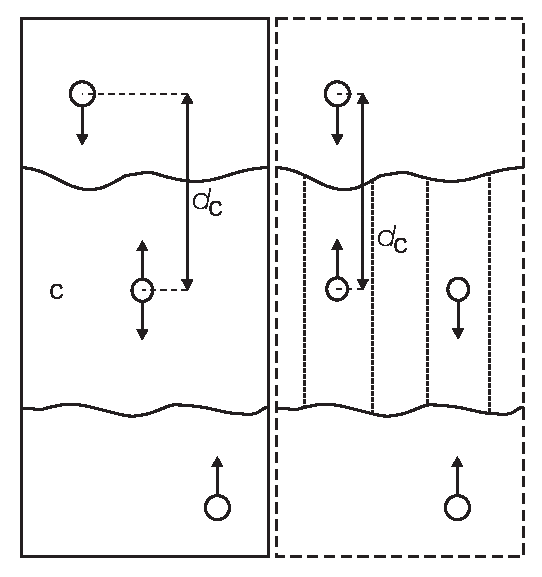
\includegraphics[width=6cm]{plots/pullref}}
\caption{Comparison of a plain center of mass reference group versus a cylinder
reference group applied to interface systems. C is the reference group.
The circles represent the center of mass of two groups plus the reference group,
$d_c$ is the reference distance.}
\label{fig:pullref} 
\end{figure}   

For a group of molecules in a periodic system, a plain reference group
might not be well-defined. An example is a water slab that is connected
periodically in $x$ and $y$, but has two liquid-vapor interfaces along $z$.
In such a setup, water molecules can evaporate from the liquid and they
will move through the vapor, through the periodic boundary, to the other
interface. Such a system is inherently periodic and there is no proper way
of defining a ``plain'' center of mass along $z$. A proper solution is to using
a cosine shaped weighting profile for all atoms in the reference group.
The profile is a cosine with a single period in the unit cell. Its phase
is optimized to give the maximum sum of weights, including mass weighting.
This provides a unique and continuous reference position that is nearly
identical to the plain center of mass position in case all atoms are all
within a half of the unit-cell length. See ref \cite{Engin2010a} for details.

When relative weights $w_i$ are used during the calculations, either
by supplying weights in the input or due to cylinder geometry
or due to cosine weighting,
the weights need to be scaled to conserve momentum:
\beq
w'_i = w_i
\left. \sum_{j=1}^N w_j \, m_j \right/ \sum_{j=1}^N w_j^2 \, m_j
\eeq
where $m_j$ is the mass of atom $j$ of the group.
The mass of the group, required for calculating the constraint force, is:
\beq
M = \sum_{i=1}^N w'_i \, m_i
\eeq
The definition of the weighted center of mass is:
\beq
\ve{r}_{com} = \left. \sum_{i=1}^N w'_i \, m_i \, \ve{r}_i \right/ M
\eeq
From the centers of mass the AFM, constraint, or umbrella force $\ve{F}_{\!com}$
on each group can be calculated.
The force on the center of mass of a group is redistributed to the atoms
as follows:
\beq
\ve{F}_{\!i} = \frac{w'_i \, m_i}{M} \, \ve{F}_{\!com}
\eeq

\subsubsection{Definition of the pull direction}

The most common setup is to pull along the direction of the vector containing
the two pull groups, this is selected with
{\tt pull-coord?-geometry = distance}. You might want to pull along a certain
vector instead, which is selected with {\tt pull-coord?-geometry = direction}.
But this can cause unwanted torque forces in the system, unless you pull against a reference group with (nearly) fixed orientation, e.g. a membrane protein embedded in a membrane along x/y while pulling along z. If your reference group does not have a fixed orientation, you should probably use
{\tt pull-coord?-geometry = direction-relative}, see \figref{pulldirrel}.
Since the potential now depends on the coordinates of two additional groups defining the orientation, the torque forces will work on these two groups.

\begin{figure}
\centerline{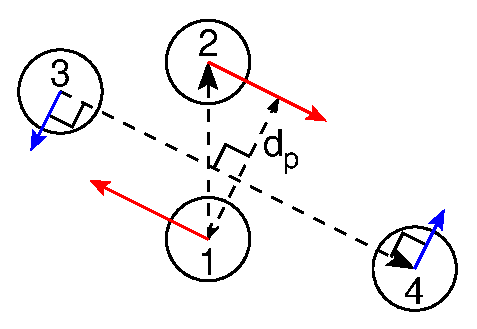
\includegraphics[width=5cm]{plots/pulldirrel}}
\caption{The pull setup for geometry {\tt direction-relative}. The ``normal'' pull groups are 1 and 2. Groups 3 and 4 define the pull direction and thus the direction of the normal pull forces (red). This leads to reaction forces (blue) on groups 3 and 4, which are perpendicular to the pull direction. Their magnitude is given by the ``normal'' pull force times the ratio of $d_p$ and the distance between groups 3 and 4.}
\label{fig:pulldirrel} 
\end{figure}   

\subsubsection{Definition of the angle and dihedral pull geometries}
Four pull groups are required for {\tt pull-coord?-geometry = angle}. In the same way as for geometries with two groups, each consecutive pair of groups
$i$ and $i+1$ define a vector connecting the COMs of groups $i$ and $i+1$. The angle is defined as the angle between the two resulting vectors.
E.g., the {\tt .mdp} option {\tt pull-coord?-groups = 1 2 2 4} defines the angle between the vector from the COM of group 1 to the COM of group 2
and the vector from the COM of group 2 to the COM of group 4.
The angle takes values in the closed interval [0, 180] deg.
For {\tt pull-coord?-geometry = angle-axis} the angle is defined with respect to a reference axis given by {\tt pull-coord?-vec} and only two groups need to be given.
The dihedral geometry requires six pull groups. These pair up in the same way as described above and so define three vectors. The dihedral angle is defined as the angle between the two
planes spanned by the two first and the two last vectors. Equivalently, the dihedral angle can be seen as the angle between the first and the third
vector when these vectors are projected onto a plane normal to the second vector (the axis vector).
As an example, consider a dihedral angle involving four groups: 1, 5, 8 and 9. Here, the {\tt .mdp} option
{\tt pull-coord?-groups = 8 1 1 5 5 9} specifies the three vectors that define the dihedral angle:
the first vector is the COM distance vector from group 8 to 1, the second vector is the COM distance vector from group 1 to 5, and the third vector is the COM distance vector from group 5 to 9.
The dihedral angle takes values in the interval (-180, 180] deg and has periodic boundaries.

\subsubsection{Limitations}
There is one theoretical limitation:
strictly speaking, constraint forces can only be calculated between
groups that are not connected by constraints to the rest of the system.
If a group contains part of a molecule of which the bond lengths
are constrained, the pull constraint and LINCS or SHAKE bond constraint
algorithms should be iterated simultaneously. This is not done in {\gromacs}.
This means that for simulations with {\tt constraints = all-bonds}
in the {\tt .mdp} file pulling is, strictly speaking,
limited to whole molecules or groups of molecules.
In some cases this limitation can be avoided by using the free energy code,
see \secref{fepmf}.
In practice, the errors caused by not iterating the two constraint
algorithms can be negligible when the pull group consists of a large
amount of atoms and/or the pull force is small.
In such cases, the constraint correction displacement of the pull group
is small compared to the bond lengths.



\section{\normindex{Enforced Rotation}}
\index{rotational pulling|see{enforced rotation}}
\index{pulling, rotational|see{enforced rotation}}
\label{sec:rotation}

\mathchardef\mhyphen="2D
\newcommand{\rotiso     }{^\mathrm{iso}}
\newcommand{\rotisopf   }{^\mathrm{iso\mhyphen pf}}
\newcommand{\rotpm      }{^\mathrm{pm}}
\newcommand{\rotpmpf    }{^\mathrm{pm\mhyphen pf}}
\newcommand{\rotrm      }{^\mathrm{rm}}
\newcommand{\rotrmpf    }{^\mathrm{rm\mhyphen pf}}
\newcommand{\rotrmtwo   }{^\mathrm{rm2}}
\newcommand{\rotrmtwopf }{^\mathrm{rm2\mhyphen pf}}
\newcommand{\rotflex    }{^\mathrm{flex}}
\newcommand{\rotflext   }{^\mathrm{flex\mhyphen t}}
\newcommand{\rotflextwo }{^\mathrm{flex2}}
\newcommand{\rotflextwot}{^\mathrm{flex2\mhyphen t}}

This module can be used to enforce the rotation of a group of atoms, as {\eg}
a protein subunit. There are a variety of rotation potentials, among them
complex ones that allow flexible adaptations of both the rotated subunit as
well as the local rotation axis during the simulation. An example application 
can be found in ref. \cite{Kutzner2011}.

\begin{figure}
\centerline{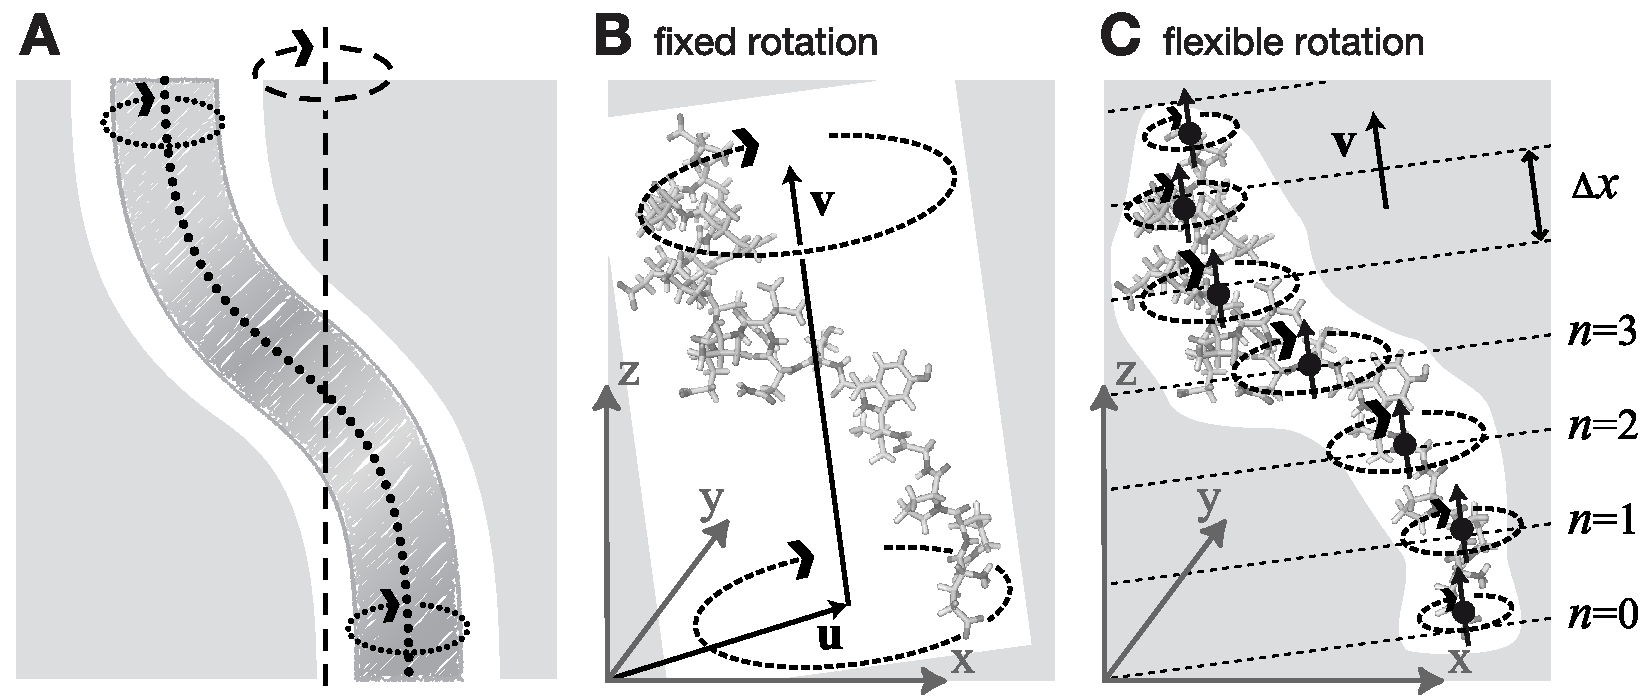
\includegraphics[width=13cm]{plots/rotation.pdf}}
\caption[Fixed and flexible axis rotation]{Comparison of fixed and flexible axis
rotation. 
{\sf A:} Rotating the sketched shape inside the white tubular cavity can create
artifacts when a fixed rotation axis (dashed) is used. More realistically, the
shape would revolve like a flexible pipe-cleaner (dotted) inside the bearing (gray). 
{\sf B:} Fixed rotation around an axis \ve{v} with a pivot point
specified by the vector \ve{u}. 
{\sf C:} Subdividing the rotating fragment into slabs with separate rotation
axes ($\uparrow$) and pivot points ($\bullet$) for each slab allows for
flexibility. The distance between two slabs with indices $n$ and $n+1$ is $\Delta x$.}
\label{fig:rotation}
\end{figure}

\begin{figure}
\centerline{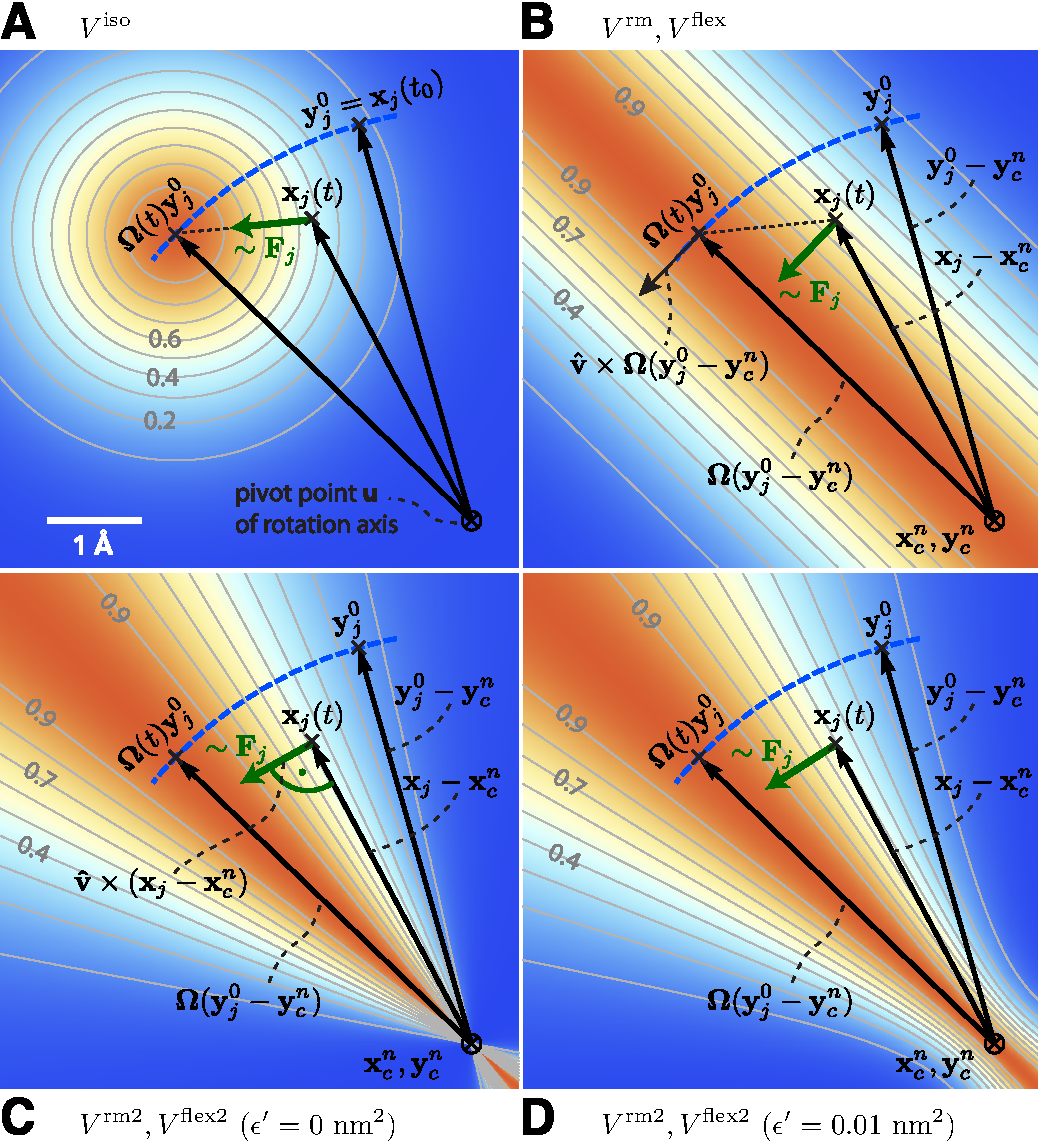
\includegraphics[width=13cm]{plots/equipotential.pdf}}
\caption{Selection of different rotation potentials and definition of notation.
All four potentials $V$ (color coded) are shown for a single atom at position
$\ve{x}_j(t)$.
{\sf A:} Isotropic potential $V\rotiso$,
{\sf B:} radial motion potential $V\rotrm$ and flexible potential
$V\rotflex$,
{\sf C--D:} radial motion\,2 potential $V\rotrmtwo$ and
flexible\,2 potential $V\rotflextwo$ for $\epsilon' = 0$\,nm$^2$ {\sf (C)}
and $\epsilon' = 0.01$\,nm$^2$ {\sf (D)}. The rotation axis is perpendicular to
the plane and marked by $\otimes$. The light gray contours indicate Boltzmann factors
$e^{-V/(k_B T)}$ in the $\ve{x}_j$-plane for $T=300$\,K and
$k=200$\,kJ/(mol$\cdot$nm$^2$). The green arrow shows the direction of the
force $\ve{F}_{\!j}$ acting on atom $j$; the blue dashed line indicates the
motion of the reference position.}
\label{fig:equipotential}
\end{figure}

\subsection{Fixed Axis Rotation}
\subsubsection{Stationary Axis with an Isotropic Potential}
In the fixed axis approach (see \figref{rotation}B), torque on a group of $N$
atoms with positions $\ve{x}_i$ (denoted ``rotation group'') is applied by
rotating a reference set of atomic positions -- usually their initial positions
$\ve{y}_i^0$ -- at a constant angular velocity $\omega$ around an axis
defined by a direction vector $\hat{\ve{v}}$ and a pivot point \ve{u}.
To that aim, each atom with position $\ve{x}_i$ is attracted by a
``virtual spring'' potential to its moving reference position
$\ve{y}_i = \mathbf{\Omega}(t) (\ve{y}_i^0 - \ve{u})$,
where $\mathbf{\Omega}(t)$ is a matrix that describes the rotation around the
axis. In the simplest case, the ``springs'' are described by a harmonic
potential,
\beq
V\rotiso = \frac{k}{2} \sum_{i=1}^{N} w_i \left[ \mathbf{\Omega}(t)
(\ve{y}_i^0 - \ve{u}) - (\ve{x}_i - \ve{u})  \right]^2 ,
\label{eqn:potiso}
\eeq
with optional mass-weighted prefactors $w_i = N \, m_i/M$ with total mass
$M = \sum_{i=1}^N m_i$.
The rotation matrix $\mathbf{\Omega}(t)$ is 
\newcommand{\omcost}{\,\xi\,}   % abbreviation
\begin{displaymath}
\mathbf{\Omega}(t) =  
\left(   
\begin{array}{ccc}
\cos\omega t + v_x^2\omcost       & v_x v_y\omcost - v_z\sin\omega t  & v_x v_z\omcost + v_y\sin\omega t\\
v_x v_y\omcost + v_z\sin\omega t  & \cos\omega t + v_y^2\omcost       & v_y v_z\omcost - v_x\sin\omega t\\
v_x v_z\omcost - v_y\sin\omega t  & v_y v_z\omcost + v_x\sin\omega t  & \cos\omega t + v_z^2\omcost     \\
\end{array}
\right) ,
\end{displaymath}
where $v_x$, $v_y$, and $v_z$ are the components of the normalized rotation vector
$\hat{\ve{v}}$, and $\omcost := 1-\cos(\omega t)$. As illustrated in
\figref{equipotential}A for a single atom $j$, the
rotation matrix $\mathbf{\Omega}(t)$ operates on the initial reference positions
$\ve{y}_j^0 = \ve{x}_j(t_0)$ of atom $j$ at $t=t_0$. At a later
time $t$, the reference position has rotated away from its initial place
(along the blue dashed line), resulting in the force
\beq
\ve{F}_{\!j}\rotiso 
= -\nabla_{\!j} \, V\rotiso 
= k \, w_j \left[
\mathbf{\Omega}(t) (\ve{y}_j^0 - \ve{u}) - (\ve{x}_j - \ve{u} ) \right] ,
\label{eqn:force_fixed}
\eeq
which is directed towards the reference position.


\subsubsection{Pivot-Free Isotropic Potential}
Instead of a fixed pivot vector \ve{u} this potential uses the center of
mass $\ve{x}_c$ of the rotation group as pivot for the rotation axis,
\beq
\ve{x}_c   = \frac{1}{M} \sum_{i=1}^N m_i \ve{x}_i 
\label{eqn:com}
\mbox{\hspace{4ex}and\hspace{4ex}}
\ve{y}_c^0 = \frac{1}{M} \sum_{i=1}^N m_i \ve{y}_i^0 \ ,
\eeq
which yields the ``pivot-free'' isotropic potential
\beq
V\rotisopf = \frac{k}{2} \sum_{i=1}^{N} w_i \left[ \mathbf{\Omega}(t)
(\ve{y}_i^0 - \ve{y}_c^0) - (\ve{x}_i - \ve{x}_c) \right]^2 ,
\label{eqn:potisopf}
\eeq
with forces
\beq
\mathbf{F}_{\!j}\rotisopf = k \, w_j 
\left[ 
\mathbf{\Omega}(t) ( \ve{y}_j^0 - \ve{y}_c^0) 
                 - ( \ve{x}_j   - \ve{x}_c )
\right] .
\label{eqn:force_isopf}
\eeq
Without mass-weighting, the pivot $\ve{x}_c$ is the geometrical center of
the group. 
\label{sec:fixed}

\subsubsection{Parallel Motion Potential Variant}
The forces generated by the isotropic potentials
(\eqnsref{potiso}{potisopf}) also contain components parallel
to the rotation axis and thereby restrain motions along the axis of either the
whole rotation group (in case of $V\rotiso$) or within
the rotation group (in case of $V\rotisopf$). For cases where
unrestrained motion along the axis is preferred, we have implemented a 
``parallel motion'' variant by eliminating all components parallel to the
rotation axis for the potential. This is achieved by projecting the distance
vectors between reference and actual positions
\beq
\ve{r}_i = \mathbf{\Omega}(t) (\ve{y}_i^0 - \ve{u}) - (\ve{x}_i - \ve{u})
\eeq
onto the plane perpendicular to the rotation vector,
\beq
\label{eqn:project}
\ve{r}_i^\perp :=  \ve{r}_i - (\ve{r}_i \cdot \hat{\ve{v}})\hat{\ve{v}} \ ,
\eeq
yielding
\bea
\nonumber
V\rotpm &=& \frac{k}{2} \sum_{i=1}^{N} w_i ( \ve{r}_i^\perp )^2 \\
        &=& \frac{k}{2} \sum_{i=1}^{N} w_i
 \left\lbrace
 \mathbf{\Omega}(t)
   (\ve{y}_i^0 - \ve{u}) - (\ve{x}_i - \ve{u})  \right. \nonumber \\
&& \left. - \left\lbrace
\left[ \mathbf{\Omega}(t)(\ve{y}_i^0 - \ve{u}) - (\ve{x}_i - \ve{u}) \right] \cdot\hat{\ve{v}}
  \right\rbrace\hat{\ve{v}} \right\rbrace^2 ,
\label{eqn:potpm}
\eea
and similarly
\beq
\ve{F}_{\!j}\rotpm = k \, w_j \, \ve{r}_j^\perp .
\label{eqn:force_pm}
\eeq

\subsubsection{Pivot-Free Parallel Motion Potential}
Replacing in \eqnref{potpm} the fixed pivot \ve{u} by the center 
of mass $\ve{x_c}$ yields the pivot-free variant of the parallel motion
potential. With
\beq
\ve{s}_i = \mathbf{\Omega}(t) (\ve{y}_i^0 - \ve{y}_c^0) - (\ve{x}_i - \ve{x}_c)
\eeq
the respective potential and forces are
\bea
V\rotpmpf &=& \frac{k}{2} \sum_{i=1}^{N} w_i ( \ve{s}_i^\perp )^2 \ , \\
\label{eqn:potpmpf}
\ve{F}_{\!j}\rotpmpf &=& k \, w_j \, \ve{s}_j^\perp .
\label{eqn:force_pmpf}
\eea

\subsubsection{Radial Motion Potential}
In the above variants, the minimum of the rotation potential is either a single
point at the reference position $\ve{y}_i$ (for the isotropic potentials) or a
single line through $\ve{y}_i$ parallel to the rotation axis (for the
parallel motion potentials). As a result, radial forces restrict radial motions
of the atoms. The two subsequent types of rotation potentials, $V\rotrm$
and $V\rotrmtwo$, drastically reduce or even eliminate this effect. The first
variant, $V\rotrm$ (\figref{equipotential}B), eliminates all force
components parallel to the vector connecting the reference atom and the
rotation axis,
\beq
V\rotrm = \frac{k}{2} \sum_{i=1}^{N} w_i \left[
\ve{p}_i
\cdot(\ve{x}_i - \ve{u}) \right]^2 ,
\label{eqn:potrm}
\eeq
with
\beq
\ve{p}_i := 
\frac{\hat{\ve{v}}\times \mathbf{\Omega}(t) (\ve{y}_i^0 - \ve{u})} {\| \hat{\ve{v}}\times \mathbf{\Omega}(t) (\ve{y}_i^0 - \ve{u})\|} \ .
\eeq
This variant depends only on the distance $\ve{p}_i \cdot (\ve{x}_i -
\ve{u})$ of atom $i$ from the plane spanned by $\hat{\ve{v}}$ and
$\mathbf{\Omega}(t)(\ve{y}_i^0 - \ve{u})$. The resulting force is
\beq
\mathbf{F}_{\!j}\rotrm =
 -k \, w_j \left[ \ve{p}_j\cdot(\ve{x}_j - \ve{u}) \right] \,\ve{p}_j \,  .
\label{eqn:potrm_force}
\eeq

\subsubsection{Pivot-Free Radial Motion Potential}
Proceeding similar to the pivot-free isotropic potential yields a pivot-free
version of the above potential. With
\beq
\ve{q}_i := 
\frac{\hat{\ve{v}}\times \mathbf{\Omega}(t) (\ve{y}_i^0 - \ve{y}_c^0)} {\| \hat{\ve{v}}\times \mathbf{\Omega}(t) (\ve{y}_i^0 - \ve{y}_c^0)\|} \, ,
\eeq
the potential and force for the pivot-free variant of the radial motion potential read
\bea
V\rotrmpf & = & \frac{k}{2} \sum_{i=1}^{N} w_i \left[
\ve{q}_i
\cdot(\ve{x}_i - \ve{x}_c)
\right]^2 \, , \\
\label{eqn:potrmpf}
\mathbf{F}_{\!j}\rotrmpf & = &
 -k \, w_j \left[ \ve{q}_j\cdot(\ve{x}_j - \ve{x}_c) \right] \,\ve{q}_j 
 + k   \frac{m_j}{M} \sum_{i=1}^{N} w_i \left[
 \ve{q}_i\cdot(\ve{x}_i - \ve{x}_c) \right]\,\ve{q}_i \, .
\label{eqn:potrmpf_force}
\eea

\subsubsection{Radial Motion 2 Alternative Potential}
As seen in \figref{equipotential}B, the force resulting from
$V\rotrm$ still contains a small, second-order radial component. In most
cases, this perturbation is tolerable; if not, the following
alternative, $V\rotrmtwo$, fully eliminates the radial contribution to the
force, as depicted in \figref{equipotential}C,
\beq
V\rotrmtwo = 
\frac{k}{2} \sum_{i=1}^{N} w_i\, 
\frac{\left[ (\hat{\ve{v}} \times ( \ve{x}_i - \ve{u} ))
\cdot \mathbf{\Omega}(t)(\ve{y}_i^0 - \ve{u}) \right]^2}
{\| \hat{\ve{v}} \times (\ve{x}_i - \ve{u}) \|^2 +
\epsilon'} \, ,
\label{eqn:potrm2}
\eeq
where a small parameter $\epsilon'$ has been introduced to avoid singularities.
For $\epsilon'=0$\,nm$^2$, the equipotential planes are spanned by $\ve{x}_i -
\ve{u}$ and $\hat{\ve{v}}$, yielding a force 
perpendicular to $\ve{x}_i - \ve{u}$, thus not contracting or
expanding structural parts that moved away from or toward the rotation axis.

Choosing a small positive  $\epsilon'$ ({\eg},
$\epsilon'=0.01$\,nm$^2$, \figref{equipotential}D) in the denominator of
\eqnref{potrm2} yields a well-defined potential and continuous forces also 
close to the rotation axis, which is not the case for $\epsilon'=0$\,nm$^2$ 
(\figref{equipotential}C). With
\bea
\ve{r}_i & := & \mathbf{\Omega}(t)(\ve{y}_i^0 - \ve{u})\\
\ve{s}_i & := & \frac{\hat{\ve{v}} \times (\ve{x}_i -
\ve{u} ) }{ \| \hat{\ve{v}} \times (\ve{x}_i - \ve{u})
\| } \equiv \; \Psi_{i} \;\; {\hat{\ve{v}} \times
(\ve{x}_i-\ve{u} ) }\\
\Psi_i^{*}   & := & \frac{1}{ \| \hat{\ve{v}} \times
(\ve{x}_i-\ve{u}) \|^2 + \epsilon'}
\eea
the force on atom $j$ reads
\beq
\ve{F}_{\!j}\rotrmtwo  = 
- k\; 
\left\lbrace w_j\;
(\ve{s}_j\cdot\ve{r}_{\!j})\;
\left[ \frac{\Psi_{\!j}^*   }{\Psi_{\!j}  }  \ve{r}_{\!j} 
     - \frac{\Psi_{\!j}^{*2}}{\Psi_{\!j}^3}
     (\ve{s}_j\cdot\ve{r}_{\!j})\ve{s}_j \right]
\right\rbrace \times \hat{\ve{v}} .
\label{eqn:potrm2_force}
\eeq

\subsubsection{Pivot-Free Radial Motion 2 Potential}
The pivot-free variant of the above potential is
\beq
V\rotrmtwopf = 
\frac{k}{2} \sum_{i=1}^{N} w_i\, 
\frac{\left[ (\hat{\ve{v}} \times ( \ve{x}_i - \ve{x}_c ))
\cdot \mathbf{\Omega}(t)(\ve{y}_i^0 - \ve{y}_c) \right]^2}
{\| \hat{\ve{v}} \times (\ve{x}_i - \ve{x}_c) \|^2 +
\epsilon'} \, .
\label{eqn:potrm2pf}
\eeq
With
\bea
\ve{r}_i & := & \mathbf{\Omega}(t)(\ve{y}_i^0 - \ve{y}_c)\\
\ve{s}_i & := & \frac{\hat{\ve{v}} \times (\ve{x}_i -
\ve{x}_c ) }{ \| \hat{\ve{v}} \times (\ve{x}_i - \ve{x}_c)
\| } \equiv \; \Psi_{i} \;\; {\hat{\ve{v}} \times
(\ve{x}_i-\ve{x}_c ) }\\ \Psi_i^{*}   & := & \frac{1}{ \| \hat{\ve{v}} \times
(\ve{x}_i-\ve{x}_c) \|^2 + \epsilon'}
\eea
the force on atom $j$ reads
\bea
\nonumber
\ve{F}_{\!j}\rotrmtwopf & = &
- k\; 
\left\lbrace w_j\;
(\ve{s}_j\cdot\ve{r}_{\!j})\;
\left[ \frac{\Psi_{\!j}^*   }{\Psi_{\!j}  } \ve{r}_{\!j} 
     - \frac{\Psi_{\!j}^{*2}}{\Psi_{\!j}^3}
     (\ve{s}_j\cdot\ve{r}_{\!j})\ve{s}_j \right]
\right\rbrace \times \hat{\ve{v}}\\
     & &
+ k\;\frac{m_j}{M} \left\lbrace \sum_{i=1}^{N}
w_i\;(\ve{s}_i\cdot\ve{r}_i) \; 
\left[ \frac{\Psi_i^*   }{\Psi_i  }  \ve{r}_i
     - \frac{\Psi_i^{*2}}{\Psi_i^3} (\ve{s}_i\cdot\ve{r}_i )\;
     \ve{s}_i \right] \right\rbrace \times \hat{\ve{v}} \, .
\label{eqn:potrm2pf_force}
\eea

\subsection{Flexible Axis Rotation}
As sketched in \figref{rotation}A--B, the rigid body behavior of
the fixed axis rotation scheme is a drawback for many applications. In
particular, deformations of the rotation group are suppressed when the
equilibrium atom positions directly depend on the reference positions. 
To avoid this limitation, \eqnsref{potrmpf}{potrm2pf}
will now be generalized towards a ``flexible axis'' as sketched in
\figref{rotation}C. This will be achieved by subdividing the
rotation group into a set of equidistant slabs perpendicular to
the rotation vector, and by applying a separate rotation potential to each
of these slabs. \figref{rotation}C shows the midplanes of the slabs 
as dotted straight lines and the centers as thick black dots.

To avoid discontinuities in the potential and in the forces, we define
``soft slabs'' by weighing the contributions of each
slab $n$ to the total potential function $V\rotflex$ by a Gaussian
function
\beq
\label{eqn:gaussian}
g_n(\ve{x}_i) = \Gamma \ \mbox{exp} \left(
-\frac{\beta_n^2(\ve{x}_i)}{2\sigma^2}  \right) ,
\eeq
centered at the midplane of the $n$th slab. Here $\sigma$ is the width
of the Gaussian function, $\Delta x$ the distance between adjacent slabs, and
\beq
\beta_n(\ve{x}_i) := \ve{x}_i \cdot \hat{\ve{v}} - n \, \Delta x \, .
\eeq
%
\begin{figure}
\centerline{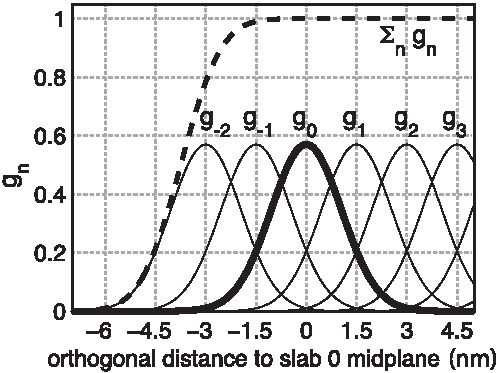
\includegraphics[width=6.5cm]{plots/gaussians.pdf}}
\caption{Gaussian functions $g_n$ centered at $n \, \Delta x$ for a slab
distance $\Delta x = 1.5$ nm and $n \geq -2$. Gaussian function $g_0$ is
highlighted in bold; the dashed line depicts the sum of the shown Gaussian
functions.}
\label{fig:gaussians}
\end{figure}
%
A most convenient choice is $\sigma = 0.7 \Delta x$ and
\begin{displaymath}
1/\Gamma = \sum_{n \in Z}
\mbox{exp}
\left(-\frac{(n - \frac{1}{4})^2}{2\cdot 0.7^2}\right)
\approx 1.75464 \, ,
\end{displaymath}
which yields a nearly constant sum, essentially independent of $\ve{x}_i$
(dashed line in \figref{gaussians}), {\ie},
\beq
\sum_{n \in Z} g_n(\ve{x}_i) =  1 + \epsilon(\ve{x}_i) \, ,
\label{eqn:normal}
\eeq
with $ | \epsilon(\ve{x}_i) | < 1.3\cdot 10^{-4}$. This choice also
implies that the individual contributions to the force from the slabs add up to
unity such that no further normalization is required.

To each slab center $\ve{x}_c^n$, all atoms contribute by their
Gaussian-weighted (optionally also mass-weighted) position vectors 
$g_n(\ve{x}_i) \, \ve{x}_i$. The
instantaneous slab centers $\ve{x}_c^n$ are calculated from the
current positions $\ve{x}_i$,
\beq
\label{eqn:defx0} 
\ve{x}_c^n =
\frac{\sum_{i=1}^N g_n(\ve{x}_i) \, m_i \, \ve{x}_i}
     {\sum_{i=1}^N g_n(\ve{x}_i) \, m_i} \, ,\\
\eeq
while the reference centers $\ve{y}_c^n$ are calculated from the reference 
positions $\ve{y}_i^0$,
\beq
\label{eqn:defy0}
\ve{y}_c^n =
\frac{\sum_{i=1}^N g_n(\ve{y}_i^0) \, m_i \, \ve{y}_i^0}
     {\sum_{i=1}^N g_n(\ve{y}_i^0) \, m_i} \, .
\eeq
Due to the rapid decay of $g_n$, each slab
will essentially involve contributions from atoms located within $\approx
3\Delta x$ from the slab center only.

\subsubsection{Flexible Axis Potential}
We consider two flexible axis variants. For the first variant,
the slab segmentation procedure with Gaussian weighting is applied to the radial 
motion potential (\eqnref{potrmpf}\,/\,\figref{equipotential}B),
yielding as the contribution of slab $n$
\begin{displaymath}
V^n = 
\frac{k}{2} \sum_{i=1}^{N} w_i \, g_n(\ve{x}_i) 
\left[
\ve{q}_i^n
\cdot
 (\ve{x}_i - \ve{x}_c^n) 
\right]^2  ,
\label{eqn:flexpot}
\end{displaymath}
and a total potential function
\beq 
V\rotflex = \sum_n V^n \, .
\label{eqn:potflex}
\eeq
Note that the global center of mass $\ve{x}_c$ used in
\eqnref{potrmpf} is now replaced by $\ve{x}_c^n$, the center of mass of
the slab. With
\bea
\ve{q}_i^n & := & \frac{\hat{\ve{v}} \times
\mathbf{\Omega}(t)(\ve{y}_i^0 - \ve{y}_c^n) }{ \| \hat{\ve{v}}
\times \mathbf{\Omega}(t)(\ve{y}_i^0 - \ve{y}_c^n) \| } \\
b_i^n         & := & \ve{q}_i^n \cdot (\ve{x}_i - \ve{x}_c^n) \, ,
\eea
the resulting force on atom $j$ reads
\bea
\nonumber\hspace{-15mm}
\ve{F}_{\!j}\rotflex &=&
- \, k \, w_j \sum_n g_n(\ve{x}_j) \, b_j^n \left\lbrace  \ve{q}_j^n -
b_j^n \frac{\beta_n(\ve{x}_j)}{2\sigma^2} \hat{\ve{v}} \right\rbrace \\ & &
+ \, k \, m_j \sum_n \frac{g_n(\ve{x}_j)}{\sum_h g_n(\ve{x}_h)}
\sum_{i=1}^{N} w_i \, g_n(\ve{x}_i) \, b_i^n \left\lbrace 
\ve{q}_i^n -\frac{\beta_n(\ve{x}_j)}{\sigma^2}
\left[ \ve{q}_i^n \cdot (\ve{x}_j - \ve{x}_c^n )\right]
\hat{\ve{v}} \right\rbrace .
\label{eqn:potflex_force}
\eea
%
Note that for $V\rotflex$, as defined, the slabs are fixed in space and so
are the reference centers $\ve{y}_c^n$. If during the simulation the
rotation group moves too far in $\ve{v}$ direction, it may enter a
region where -- due to the lack of nearby reference positions -- no reference
slab centers are defined, rendering the potential evaluation impossible. 
We therefore have included a slightly modified version of this potential that
avoids this problem by attaching the midplane of slab $n=0$ to the center of mass 
of the rotation group, yielding slabs that move with the rotation group. 
This is achieved by subtracting the center of mass $\ve{x}_c$ of the
group from the positions, 
\beq
\tilde{\ve{x}}_i = \ve{x}_i - \ve{x}_c \, , \mbox{\ \ \ and \ \ } 
\tilde{\ve{y}}_i^0 = \ve{y}_i^0 - \ve{y}_c^0 \, ,
\label{eqn:trafo} 
\eeq
such that
\bea
V\rotflext 
  & = & \frac{k}{2} \sum_n \sum_{i=1}^{N} w_i \, g_n(\tilde{\ve{x}}_i)
  \left[ \frac{\hat{\ve{v}} \times \mathbf{\Omega}(t)(\tilde{\ve{y}}_i^0
  - \tilde{\ve{y}}_c^n) }{ \| \hat{\ve{v}} \times
\mathbf{\Omega}(t)(\tilde{\ve{y}}_i^0 -
\tilde{\ve{y}}_c^n) \| }
\cdot
 (\tilde{\ve{x}}_i - \tilde{\ve{x}}_c^n) 
\right]^2 .
\label{eqn:potflext}
\eea
To simplify the force derivation, and for efficiency reasons, we here assume
$\ve{x}_c$ to be constant, and thus $\partial \ve{x}_c / \partial x =
\partial \ve{x}_c / \partial y = \partial \ve{x}_c / \partial z = 0$. The
resulting force error is small (of order $O(1/N)$ or $O(m_j/M)$ if
mass-weighting is applied) and can therefore be tolerated. With this assumption,
the forces $\ve{F}\rotflext$ have the same form as
\eqnref{potflex_force}.

\subsubsection{Flexible Axis 2 Alternative Potential}
In this second variant, slab segmentation is applied to $V\rotrmtwo$
(\eqnref{potrm2pf}), resulting in a flexible axis potential without radial
force contributions (\figref{equipotential}C),
\beq
V\rotflextwo = 
\frac{k}{2} \sum_{i=1}^{N} \sum_n w_i\,g_n(\ve{x}_i) 
\frac{\left[ (\hat{\ve{v}} \times ( \ve{x}_i - \ve{x}_c^n ))
\cdot \mathbf{\Omega}(t)(\ve{y}_i^0 - \ve{y}_c^n) \right]^2}
{\| \hat{\ve{v}} \times (\ve{x}_i - \ve{x}_c^n) \|^2 +
\epsilon'} \, .
\label{eqn:potflex2}
\eeq
With
\bea
\ve{r}_i^n & := & \mathbf{\Omega}(t)(\ve{y}_i^0 - \ve{y}_c^n)\\
\ve{s}_i^n & := & \frac{\hat{\ve{v}} \times (\ve{x}_i -
\ve{x}_c^n ) }{ \| \hat{\ve{v}} \times (\ve{x}_i - \ve{x}_c^n)
\| } \equiv \; \psi_{i} \;\; {\hat{\ve{v}} \times (\ve{x}_i-\ve{x}_c^n ) }\\
\psi_i^{*}     & := & \frac{1}{ \| \hat{\ve{v}} \times (\ve{x}_i-\ve{x}_c^n) \|^2 + \epsilon'}\\ 
W_j^n          & := & \frac{g_n(\ve{x}_j)\,m_j}{\sum_h g_n(\ve{x}_h)\,m_h}\\
\ve{S}^n   & := & 
\sum_{i=1}^{N} w_i\;g_n(\ve{x}_i)
\; (\ve{s}_i^n\cdot\ve{r}_i^n)
\left[ \frac{\psi_i^*   }{\psi_i  }  \ve{r}_i^n
     - \frac{\psi_i^{*2}}{\psi_i^3} (\ve{s}_i^n\cdot\ve{r}_i^n )\;
     \ve{s}_i^n \right] \label{eqn:Sn}
\eea
the force on atom $j$ reads
\bea
\nonumber
\ve{F}_{\!j}\rotflextwo & = &
- k\; 
\left\lbrace \sum_n w_j\;g_n(\ve{x}_j)\;
(\ve{s}_j^n\cdot\ve{r}_{\!j}^n)\;
\left[ \frac{\psi_j^*   }{\psi_j  }  \ve{r}_{\!j}^n 
     - \frac{\psi_j^{*2}}{\psi_j^3} (\ve{s}_j^n\cdot\ve{r}_{\!j}^n)\;
     \ve{s}_{\!j}^n \right] \right\rbrace \times \hat{\ve{v}} \\
\nonumber
& &
+ k \left\lbrace \sum_n W_{\!j}^n \, \ve{S}^n \right\rbrace \times
\hat{\ve{v}}
- k \left\lbrace \sum_n W_{\!j}^n \; \frac{\beta_n(\ve{x}_j)}{\sigma^2} \frac{1}{\psi_j}\;\; 
\ve{s}_j^n \cdot 
\ve{S}^n \right\rbrace \hat{\ve{v}}\\ 
& & 
+ \frac{k}{2} \left\lbrace \sum_n w_j\;g_n(\ve{x}_j)
\frac{\beta_n(\ve{x}_j)}{\sigma^2} 
\frac{\psi_j^*}{\psi_j^2}( \ve{s}_j^n \cdot \ve{r}_{\!j}^n )^2 \right\rbrace
\hat{\ve{v}} .
\label{eqn:potflex2_force}
\eea

Applying transformation (\ref{eqn:trafo}) yields a ``translation-tolerant''
version of the flexible\,2 potential, $V\rotflextwot$. Again,
assuming that $\partial \ve{x}_c / \partial x$,  $\partial \ve{x}_c /
\partial y$, $\partial \ve{x}_c / \partial z$ are small, the
resulting equations for $V\rotflextwot$ and $\ve{F}\rotflextwot$ are
similar to those of $V\rotflextwo$ and $\ve{F}\rotflextwo$.

\subsection{Usage}
To apply enforced rotation, the particles $i$ that are to
be subjected to one of the rotation potentials are defined via index groups
{\tt rot-group0}, {\tt rot-group1}, etc., in the {\tt .mdp} input file. 
The reference positions $\ve{y}_i^0$ are
read from a special {\tt .trr} file provided to {\tt grompp}. If no such file is found,
$\ve{x}_i(t=0)$ are used as reference positions and written to {\tt .trr} such
that they can be used for subsequent setups. All parameters of the potentials
such as $k$, $\epsilon'$, etc. (\tabref{vars}) are provided as {\tt .mdp}
parameters; {\tt rot-type} selects the type of the potential. 
The option {\tt rot-massw} allows to choose whether or not to use
mass-weighted averaging. 
For the flexible potentials, a cutoff value $g_n^\mathrm{min}$ 
(typically  $g_n^\mathrm{min}=0.001$) makes shure that only
significant contributions to $V$ and \ve{F} are evaluated, {\ie} terms with 
$g_n(\ve{x}) < g_n^\mathrm{min}$ are omitted.
\tabref{quantities} summarizes observables that are written
to additional output files and which are described below.


\begin{table}[tbp]
\caption{Parameters used by the various rotation potentials.
{\sf x}'s indicate which parameter is actually used for a given potential.}
%\small

\newcommand{\kunit}{$\frac{\mathrm{kJ}}{\mathrm{mol} \cdot \mathrm{nm}^2}$}
\newcommand{\smtt}[1]{{\hspace{-0.5ex}\small #1\hspace{-0.5ex}}}
\label{tab:vars}
\begin{center}
\begin{tabular}{l>{$}l<{$}rccccccc}
\hline
parameter           &               &                      & $k$      & $\hat{\ve{v}}$ & $\ve{u}$     & $\omega$    & $\epsilon'$ & $\Delta x$        & $g_n^\mathrm{min}$ \\
\multicolumn{3}{l}{{\tt .mdp} input variable name}         & \smtt{k} & \smtt{vec}     & \smtt{pivot} & \smtt{rate} & \smtt{eps}  & \smtt{slab-dist}  & \smtt{min-gauss}   \\
unit                &               &                      & \kunit   & -              & nm           & $^\circ$/ps & nm$^2$      & nm                & \,-\,              \\[1mm]
\hline \multicolumn{2}{l}{fixed axis potentials:} & eqn.\\
isotropic           & V\rotiso      & (\ref{eqn:potiso})   & {\sf x}  & {\sf x}        & {\sf x}      & {\sf x}     & -           & -                 &  -                 \\
--- pivot-free      & V\rotisopf    & (\ref{eqn:potisopf}) & {\sf x}  & {\sf x}        & -            & {\sf x}     & -           & -                 &  -                 \\
parallel motion     & V\rotpm       & (\ref{eqn:potpm})    & {\sf x}  & {\sf x}        & {\sf x}      & {\sf x}     & -           & -                 &  -                 \\
--- pivot-free      & V\rotpmpf     & (\ref{eqn:potpmpf})  & {\sf x}  & {\sf x}        & -            & {\sf x}     & -           & -                 &  -                 \\
radial motion       & V\rotrm       & (\ref{eqn:potrm})    & {\sf x}  & {\sf x}        & {\sf x}      & {\sf x}     & -           & -                 &  -                 \\
--- pivot-free      & V\rotrmpf     & (\ref{eqn:potrmpf})  & {\sf x}  & {\sf x}        & -            & {\sf x}     & -           & -                 &  -                 \\
radial motion\,2    & V\rotrmtwo    & (\ref{eqn:potrm2})   & {\sf x}  & {\sf x}        & {\sf x}      & {\sf x}     & {\sf x}     & -                 &  -                 \\
--- pivot-free      & V\rotrmtwopf  & (\ref{eqn:potrm2pf}) & {\sf x}  & {\sf x}        & -            & {\sf x}     & {\sf x}     & -                 &  -                 \\ \hline
\multicolumn{2}{l}{flexible axis potentials:}  & eqn.\\
flexible            & V\rotflex     & (\ref{eqn:potflex})  & {\sf x}  & {\sf x}        & -            & {\sf x}     & -           & {\sf x}           &  {\sf x}           \\
--- transl. tol.    & V\rotflext    & (\ref{eqn:potflext}) & {\sf x}  & {\sf x}        & -            & {\sf x}     & -           & {\sf x}           &  {\sf x}           \\
flexible\,2         & V\rotflextwo  & (\ref{eqn:potflex2}) & {\sf x}  & {\sf x}        & -            & {\sf x}     & {\sf x}     & {\sf x}           &  {\sf x}           \\
--- transl. tol.    & V\rotflextwot &  -                   & {\sf x}  & {\sf x}        & -            & {\sf x}     & {\sf x}     & {\sf x}           &  {\sf x}           \\
\hline
\end{tabular}
\end{center}
\end{table}

\begin{table}
\caption{Quantities recorded in output files during enforced rotation simulations.
All slab-wise data is written every {\tt nstsout} steps, other rotation data every {\tt nstrout} steps.}
\label{tab:quantities}
\begin{center}
\begin{tabular}{llllcc}
\hline
quantity                                             & unit    & equation                          & output file     & fixed   & flexible\\ \hline
$V(t)$                                               & kJ/mol  & see \ref{tab:vars}                & {\tt rotation}  & {\sf x} & {\sf x} \\
$\theta_\mathrm{ref}(t)$                             & degrees & $\theta_\mathrm{ref}(t)=\omega t$ & {\tt rotation}  & {\sf x} & {\sf x} \\
$\theta_\mathrm{av}(t)$                              & degrees & (\ref{eqn:avangle})               & {\tt rotation}  & {\sf x} & -       \\
$\theta_\mathrm{fit}(t)$, $\theta_\mathrm{fit}(t,n)$ & degrees & (\ref{eqn:rmsdfit})               & {\tt rotangles} & -       & {\sf x} \\
$\ve{y}_0(n)$, $\ve{x}_0(t,n)$                       & nm      & (\ref{eqn:defx0}, \ref{eqn:defy0})& {\tt rotslabs}  & -       & {\sf x} \\
$\tau(t)$                                            & kJ/mol  & (\ref{eqn:torque})                & {\tt rotation}  & {\sf x} & -       \\
$\tau(t,n)$                                          & kJ/mol  & (\ref{eqn:torque})                & {\tt rottorque} & -       & {\sf x} \\ \hline
\end{tabular}
\end{center}
\end{table}


\subsubsection*{Angle of Rotation Groups: Fixed Axis}
For fixed axis rotation, the average angle $\theta_\mathrm{av}(t)$ of the 
group relative to the reference group is determined via the distance-weighted
angular deviation of all rotation group atoms from their reference positions,
\beq
\theta_\mathrm{av} = \left. \sum_{i=1}^{N} r_i \ \theta_i \right/ \sum_{i=1}^N r_i \ .
\label{eqn:avangle}
\eeq
Here, $r_i$ is the distance of the reference position to the rotation axis, and
the difference angles $\theta_i$ are determined from the atomic positions, 
projected onto a plane perpendicular to the rotation axis through pivot point
$\ve{u}$ (see \eqnref{project} for the definition of $\perp$),
\beq
\cos \theta_i = 
\frac{(\ve{y}_i-\ve{u})^\perp \cdot (\ve{x}_i-\ve{u})^\perp}
     { \| (\ve{y}_i-\ve{u})^\perp \cdot (\ve{x}_i-\ve{u})^\perp
     \| } \ .
\eeq
%
The sign of $\theta_\mathrm{av}$ is chosen such that
$\theta_\mathrm{av} > 0$ if the actual structure rotates ahead of the reference.

\subsubsection*{Angle of Rotation Groups: Flexible Axis}
For flexible axis rotation, two outputs are provided, the angle of the
entire rotation group, and separate angles for the segments in the slabs.
The angle of the entire rotation group is determined by an RMSD fit 
of $\ve{x}_i$
to the reference positions $\ve{y}_i^0$ at $t=0$, yielding $\theta_\mathrm{fit}$
as the angle by which the reference has to be rotated around $\hat{\ve{v}}$ 
for the optimal fit,
\beq
\mathrm{RMSD} \big( \ve{x}_i,\ \mathbf{\Omega}(\theta_\mathrm{fit})
\ve{y}_i^0 \big) \stackrel{!}{=} \mathrm{min} \, .
\label{eqn:rmsdfit}
\eeq
To determine the local angle for each slab $n$, both reference and actual
positions are weighted with the Gaussian function of slab $n$, and 
$\theta_\mathrm{fit}(t,n)$ is calculated as in \eqnref{rmsdfit}) from the
Gaussian-weighted positions.

For all angles, the {\tt .mdp} input option {\tt rot-fit-method} controls
whether a normal RMSD fit is performed or whether for the fit each
position $\ve{x}_i$ is put at the same distance to the rotation axis as its
reference counterpart $\ve{y}_i^0$. In the latter case, the RMSD
measures only angular differences, not radial ones.


\subsubsection*{Angle Determination by Searching the Energy Minimum}
Alternatively, for {\tt rot-fit-method = potential}, the angle of the rotation 
group is determined as the angle for which the rotation potential energy is minimal.
Therefore, the used rotation potential is additionally evaluated for a set of angles
around the current reference angle. In this case, the {\tt rotangles.log} output file
contains the values of the rotation potential at the chosen set of angles, while 
{\tt rotation.xvg} lists the angle with minimal potential energy.


\subsubsection*{Torque}
\label{torque}
The torque $\ve{\tau}(t)$ exerted by the rotation potential is calculated for fixed
axis rotation via
\beq
\ve{\tau}(t) = \sum_{i=1}^{N} \ve{r}_i(t) \times \ve{f}_{\!i}^\perp(t) ,
\label{eqn:torque}
\eeq
where $\ve{r}_i(t)$ is the distance vector from the rotation axis to
$\ve{x}_i(t)$ and $\ve{f}_{\!i}^\perp(t)$ is the force component
perpendicular to $\ve{r}_i(t)$ and $\hat{\ve{v}}$. For flexible axis
rotation, torques $\ve{\tau}_{\!n}$ are calculated for each slab using the
local rotation axis of the slab and the Gaussian-weighted positions.


\section{\normindex{Electric fields}}
A pulsed and oscillating electric field can be applied according to:
\begin{equation}
E(t) = E_0 \exp\left[-\frac{(t-t_0)^2}{2\sigma^2}\right]\cos\left[\omega (t-t_0)\right]
\label{eq_efield}
\end{equation}
where $E_0$ is the field strength, the angular frequency \mbox{$\omega = 2\pi c/\lambda$}, $t_0$ is
the time at of the peak in the field strength and $\sigma$ is the with
of the pulse. Special cases occur when $\sigma$ = 0 (non-pulsed field)
and for $\omega$ is 0 (static field).

This simulated \normindex{laser}-pulse was applied to
simulations of melting ice~\cite{Caleman2008a}. A pulsed electric field may
look ike Fig.~\ref{fig:field}. In the supporting
information of that paper the impact of an applied electric field on a
system under periodic boundary conditions is analyzed. It is described
that the effective electric field under PBC is larger than the applied
field, by a factor depending on the size of the box and the dielectric
properties of molecules in the box. For a system with static dielectric
properties this factor can be corrected for. But for a system where
the dielectric varies over time, for example a membrane protein with
a pore that opens and closes during the simulatippn, this way of applying
an electric field is not useful. In such cases one can use the computational
electrophysiology protocol described in the next section (\secref{compel}).
\begin{figure}[ht]
\centerline{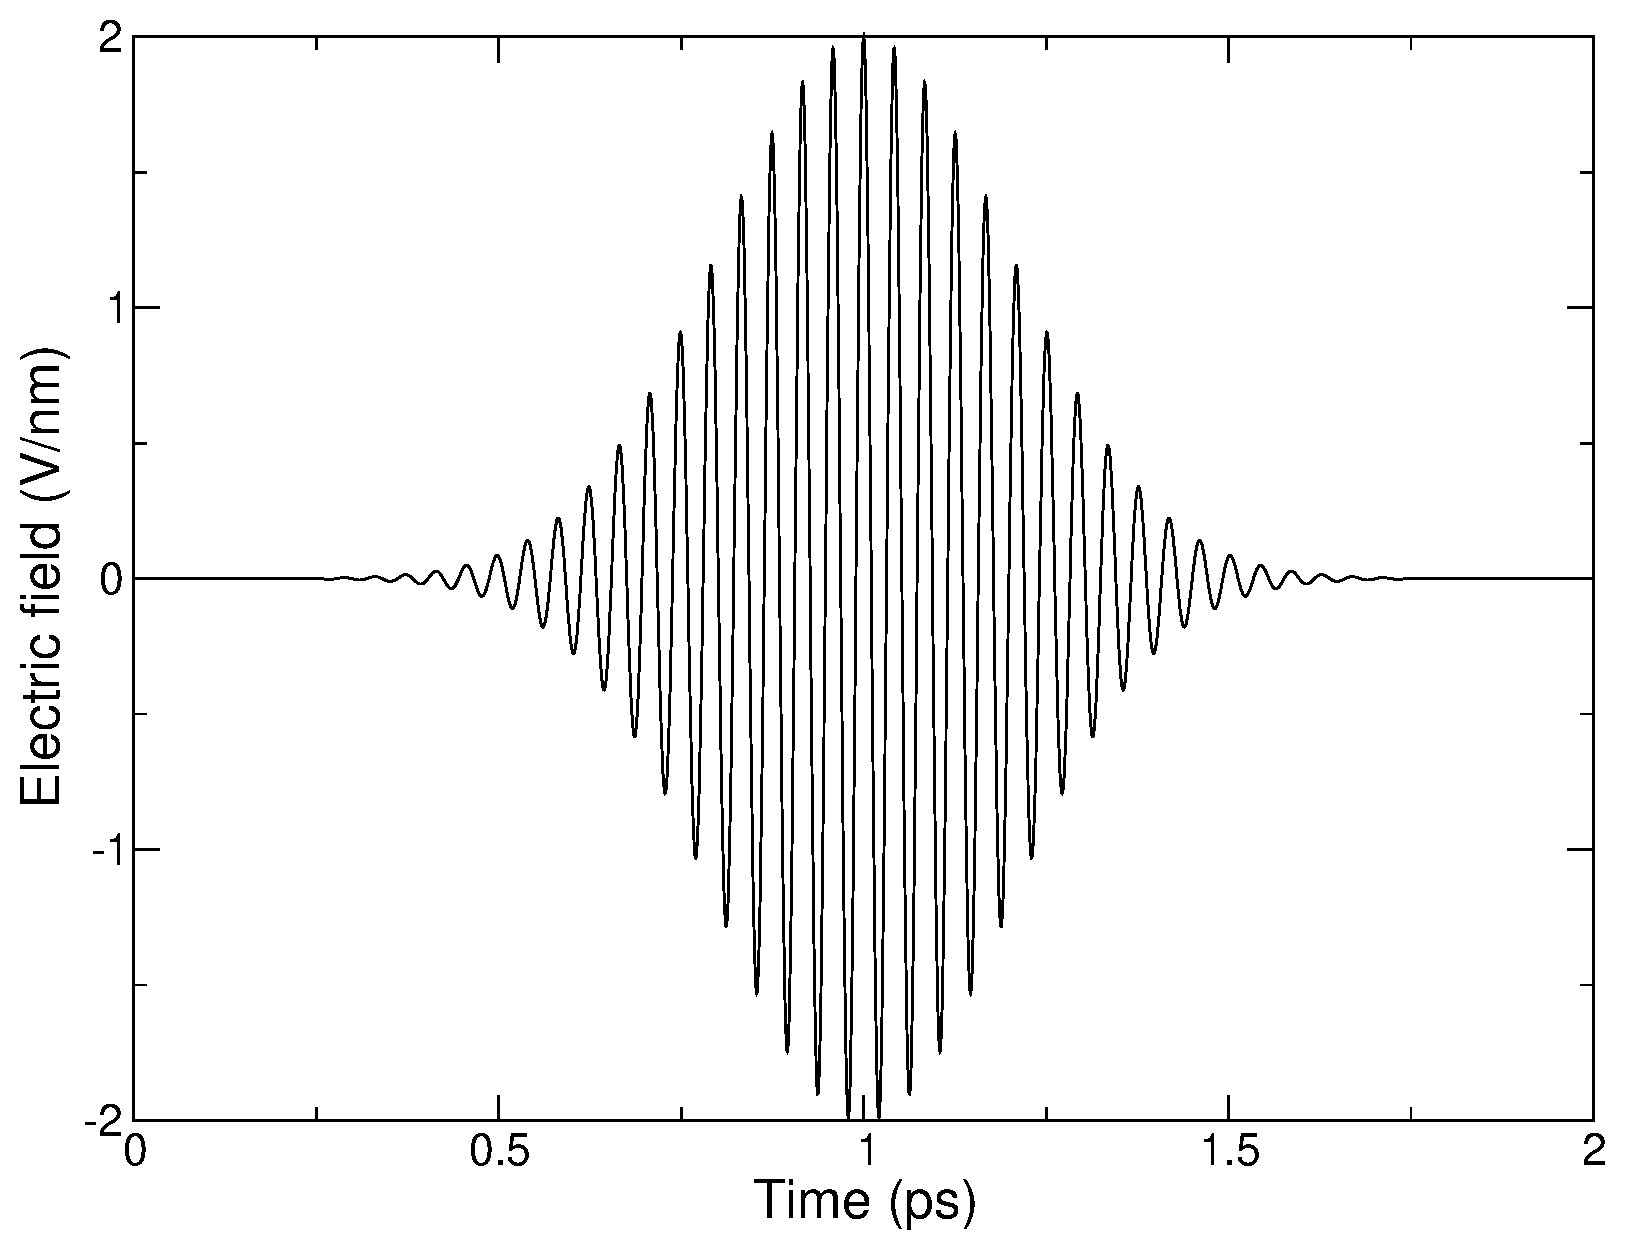
\includegraphics[width=8cm]{plots/field}}
\caption {A simulated laser pulse in GROMACS.}
\label{fig:field}
\end{figure}

Electric fields are applied when the following options are specified
in the {\tt grompp.mdp} file. You specify, in order, $E_0$, $\omega$,
$t_0$ and $\sigma$:
\begin{verbatim}
ElectricField-x = 0.04 0       0     0
\end{verbatim}
yields a static field with $E_0$ = 0.04 V/nm in the X-direction. In contrast,
\begin{verbatim}
ElectricField-x = 2.0  150     5     0
\end{verbatim}
yields an oscillating electric field with $E_0$ = 2 V/nm, $\omega$ = 150/ps and
$t_0$ = 5 ps. Finally 
\begin{verbatim}
ElectricField-x = 2.0  150     5     1
\end{verbatim}
yields an pulsed-oscillating electric field with $E_0$ = 2 V/nm, $\omega$ = 150/ps and
$t_0$ = 5 ps and $\sigma$ = 1 ps. Read more in ref.~\cite{Caleman2008a}.
Note that the input file format is changed from the undocumented older
version. A figure like Fig.~\ref{fig:field} may be produced by passing
the {\tt -field} option to {\tt gmx mdrun}.


\section{\normindex{Computational Electrophysiology}}
\label{sec:compel}

The Computational Electrophysiology (CompEL) protocol \cite{Kutzner2011b} allows the simulation of
ion flux through membrane channels, driven by transmembrane potentials or ion
concentration gradients. Just as in real cells, CompEL establishes transmembrane
potentials by sustaining a small imbalance of charges $\Delta q$ across the membrane,
which gives rise to a potential difference $\Delta U$ according to the membrane capacitance:
\beq
\Delta U = \Delta q / C_{membrane}
\eeq
The transmembrane electric field and concentration gradients are controlled by
{\tt .mdp} options, which allow the user to set reference counts for the ions on either side
of the membrane. If a difference between the actual and the reference numbers persists
over a certain time span, specified by the user, a number of ion/water pairs are
exchanged between the compartments until the reference numbers are restored.
Alongside the calculation of channel conductance and ion selectivity, CompEL simulations also
enable determination of the channel reversal potential, an important
characteristic obtained in electrophysiology experiments.

In a CompEL setup, the simulation system is divided into two compartments {\bf A} and {\bf B}
with independent ion concentrations. This is best achieved by using double bilayer systems with
a copy (or copies) of the channel/pore of interest in each bilayer (\figref{compelsetup} A, B).
If the channel axes point in the same direction, channel flux is observed
simultaneously at positive and negative potentials in this way, which is for instance
important for studying channel rectification.

\begin{figure}
\centerline{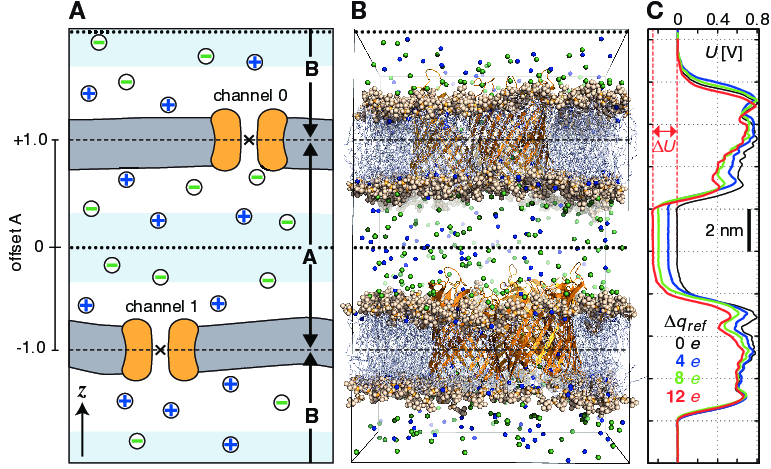
\includegraphics[width=13.5cm]{plots/compelsetup.pdf}}
\caption{Typical double-membrane setup for CompEL simulations (A, B).
Ion\,/\,water molecule exchanges will be performed as needed
between the two light blue volumes around the dotted black lines (A).
Plot (C) shows the potential difference $\Delta U$ resulting
from the selected charge imbalance $\Delta q_{ref}$ between the compartments.}
\label{fig:compelsetup}
\end{figure}

The potential difference $\Delta U$ across the membrane is easily calculated with the
{\tt gmx potential} utility. By this, the potential drop along $z$ or the
pore axis is exactly known in each time interval of the simulation (\figref{compelsetup} C).
Type and number of ions $n_i$ of charge $q_i$, traversing the channel in the simulation,
are written to the {\tt swapions.xvg} output file, from which the average channel
conductance $G$ in each interval $\Delta t$ is determined by:
\beq
G = \frac{\sum_{i} n_{i}q_{i}}{\Delta t \, \Delta U} \, .
\eeq
The ion selectivity is calculated as the number flux ratio of different species.
Best results are obtained by averaging these values over several overlapping time intervals.

The calculation of reversal potentials is best achieved using a small set of simulations in which a given
transmembrane concentration gradient is complemented with small ion imbalances of varying magnitude. For
example, if one compartment contains 1\,M salt and the other 0.1\,M, and given charge neutrality otherwise,
a set of simulations with $\Delta q = 0\,e$, $\Delta q = 2\,e$, $\Delta q = 4\,e$ could
be used. Fitting a straight line through the current-voltage relationship of all obtained
$I$-$U$ pairs near zero current will then yield $U_{rev}$.

\subsection{Usage}
The following {\tt .mdp} options control the CompEL protocol:
{\small
\begin{verbatim}
swapcoords     = Z        ; Swap positions: no, X, Y, Z
swap-frequency = 100      ; Swap attempt frequency
\end{verbatim}}
Choose {\tt Z} if your membrane is in the $xy$-plane (\figref{compelsetup}).
Ions will be exchanged between compartments depending on their $z$-positions alone.
{\tt swap-frequency} determines how often a swap attempt will be made.
This step requires that the positions of the split groups, the ions, and possibly the solvent molecules are
communicated between the parallel processes, so if chosen too small it can decrease the simulation
performance. The {\tt Position swapping} entry in the cycle and time accounting
table at the end of the {\tt md.log} file summarizes the amount of runtime spent
in the swap module.
{\small
\begin{verbatim}
split-group0   = channel0 ; Defines compartment boundary
split-group1   = channel1 ; Defines other compartment boundary
massw-split0   = no       ; use mass-weighted center?
massw-split1   = no
\end{verbatim}}
{\tt split-group0} and {\tt split-group1} are two index groups that define the boundaries
between the two compartments, which are usually the centers of the channels.
If {\tt massw-split0} or {\tt massw-split1} are set to {\tt yes}, the center of mass
of each index group is used as boundary, here in $z$-direction. Otherwise, the
geometrical centers will be used ($\times$ in \figref{compelsetup} A). If, such as here, a membrane
channel is selected as split group, the center of the channel will define the dividing
plane between the compartments (dashed horizontal lines). All index groups
must be defined in the index file.

If, to restore the requested ion counts, an ion from one compartment has to be exchanged
with a water molecule from the other compartment, then those molecules are swapped
which have the largest distance to the compartment-defining boundaries
(dashed horizontal lines). Depending on the ion concentration,
this effectively results in exchanges of molecules between the light blue volumes.
If a channel is very asymmetric in $z$-direction and would extend into one of the
swap volumes, one can offset the swap exchange plane with the {\tt bulk-offset}
parameter. A value of 0.0 means no offset $b$, values $-1.0 < b < 0$ move the
swap exchange plane closer to the lower, values $0 < b < 1.0$ closer to the upper
membrane. \figref{compelsetup} A (left) depicts that for the {\bf A} compartment.

{\small
\begin{verbatim}
solvent-group  = SOL      ; Group containing the solvent molecules
iontypes       = 3        ; Number of different ion types to control
iontype0-name  = NA       ; Group name of the ion type
iontype0-in-A  = 51       ; Reference count of ions of type 0 in A
iontype0-in-B  = 35       ; Reference count of ions of type 0 in B
iontype1-name  = K
iontype1-in-A  = 10
iontype1-in-B  = 38
iontype2-name  = CL
iontype2-in-A  = -1
iontype2-in-B  = -1
\end{verbatim}}
The group name of solvent molecules acting as exchange partners for the ions
has to be set with {\tt solvent-group}. The number of different ionic species under
control of the CompEL protocol is given by the {\tt iontypes} parameter,
while {\tt iontype0-name} gives the name of the index group containing the
atoms of this ionic species. The reference number of ions of this type 
can be set with the {\tt iontype0-in-A} and {\tt iontype0-in-B} options
for compartments {\bf A} and {\bf B}, respectively. Obviously,
the sum of {\tt iontype0-in-A} and {\tt iontype0-in-B} needs to equal the number
of ions in the group defined by {\tt iontype0-name}.
A reference number of {\tt -1} means: use the number of ions as found at the beginning
of the simulation as the reference value.

{\small
\begin{verbatim}
coupl-steps    = 10       ; Average over these many swap steps
threshold      = 1        ; Do not swap if < threshold
\end{verbatim}}
If {\tt coupl-steps} is set to 1, then the momentary ion distribution determines
whether ions are exchanged. {\tt coupl-steps} \textgreater\ 1 will use the time-average
of ion distributions over the selected number of attempt steps instead. This can be useful, for example,
when ions diffuse near compartment boundaries, which would lead to numerous unproductive
ion exchanges. A {\tt threshold} of 1 means that a swap is performed if the average ion
count in a compartment differs by at least 1 from the requested values. Higher thresholds
will lead to toleration of larger differences. Ions are exchanged until the requested
number $\pm$ the threshold is reached.

{\small
\begin{verbatim}
cyl0-r         = 5.0      ; Split cylinder 0 radius (nm)
cyl0-up        = 0.75     ; Split cylinder 0 upper extension (nm)
cyl0-down      = 0.75     ; Split cylinder 0 lower extension (nm)
cyl1-r         = 5.0      ; same for other channel
cyl1-up        = 0.75
cyl1-down      = 0.75
\end{verbatim}}
The cylinder options are used to define virtual geometric cylinders around the
channel's pore to track how many ions of which type have passed each channel.
Ions will be counted as having traveled through a channel
according to the definition of the channel's cylinder radius, upper and lower extension,
relative to the location of the respective split group. This will not affect the actual
flux or exchange, but will provide you with the ion permeation numbers across
each of the channels. Note that an ion can only be counted as passing through a particular
channel if it is detected \emph{within} the defined split cylinder in a swap step.
If {\tt swap-frequency} is chosen too high, a particular ion may be detected in compartment {\bf A}
in one swap step, and in compartment {\bf B} in the following swap step, so it will be unclear
through which of the channels it has passed.

A double-layered system for CompEL simulations can be easily prepared by
duplicating an existing membrane/channel MD system in the direction of the membrane
normal (typically $z$) with {\tt gmx editconf -translate 0 0 <l_z>}, where {\tt l_z}
is the box length in that direction. If you have already defined index groups for
the channel for the single-layered system, {\tt gmx make_ndx -n index.ndx -twin} will
provide you with the groups for the double-layered system.

To suppress large fluctuations of the membranes along the swap direction,
it may be useful to apply a harmonic potential (acting only in the swap dimension)
between each of the two channel and/or bilayer centers using umbrella pulling
(see section~\ref{sec:pull}).

\subsection*{Multimeric channels}
If a split group consists of more than one molecule, the correct PBC image of all molecules
with respect to each other has to be chosen such that the channel center can be correctly
determined. \gromacs\ assumes that the starting structure in the {\tt .tpr}
file has the correct PBC representation. Set the following environment variable
to check whether that is the case:
\begin{itemize}
\item   {\tt GMX_COMPELDUMP}: output the starting structure after it has been made whole to
        {\tt .pdb} file.
\end{itemize}


\section{Calculating a PMF using the free-energy code}
\label{sec:fepmf}
\index{potentials of mean force}
\index{free energy calculations}
The free-energy coupling-parameter approach (see~\secref{fecalc})
provides several ways to calculate potentials of mean force.
A potential of mean force between two atoms can be calculated
by connecting them with a harmonic potential or a constraint.
For this purpose there are special potentials that avoid the generation of
extra exclusions, see~\secref{excl}.
When the position of the minimum or the constraint length is 1 nm more
in state B than in state A, the restraint or constraint force is given
by $\partial H/\partial \lambda$.
The distance between the atoms can be changed as a function of $\lambda$
and time by setting {\tt delta-lambda} in the {\tt .mdp} file.
The results should be identical (although not numerically
due to the different implementations) to the results of the pull code
with umbrella sampling and constraint pulling.
Unlike the pull code, the free energy code can also handle atoms that
are connected by constraints.

Potentials of mean force can also be calculated using position restraints.
With position restraints, atoms can be linked to a position in space
with a harmonic potential (see \ssecref{positionrestraint}).
These positions can be made a function of the coupling parameter $\lambda$.
The positions for the A and the B states are supplied to {\tt grompp} with
the {\tt -r} and {\tt -rb} options, respectively.
One could use this approach to do \normindex{targeted MD};
note that we do not encourage the use of targeted MD for proteins.
A protein can be forced from one conformation to another by using
these conformations as position restraint coordinates for state A and B.
One can then slowly change $\lambda$ from 0 to 1.
The main drawback of this approach is that the conformational freedom
of the protein is severely limited by the position restraints,
independent of the change from state A to B.
Also, the protein is forced from state A to B in an almost straight line,
whereas the real pathway might be very different.
An example of a more fruitful application is a solid system or a liquid
confined between walls where one wants to measure the force required
to change the separation between the boundaries or walls.
Because the boundaries (or walls) already need to be fixed,
the position restraints do not limit the system in its sampling.

%%%%%%%%%%%%%%%%%%%%%%%%%%%%%%%%%%%%%%%%%%%%%%%%%%%%%%%%%%%%%%%%%%%%%%%%%%%%%%%
%%%%%%%%%%%%%%%%%%%%%%%%%%%%%%%%%%%%%%%%%%%%%%%%%%%%%%%%%%%%%%%%%%%%%%%%%%%%%%%
%%%%%%%%%%%%%%%%%%%%%%%%%%%%%%%%%%%%%%%%%%%%%%%%%%%%%%%%%%%%%%%%%%%%%%%%%%%%%%%
\newcommand{\amine}{\sf -NH$_2$}
\newcommand{\amines}{\sf -NH-}
\newcommand{\aminep}{\sf -NH$_3^+$}
\section{Removing fastest \swapindex{degrees of}{freedom}}
\label{sec:rmfast}
The maximum time step in MD simulations is limited by the smallest
oscillation period that can be found in the simulated
system. Bond-stretching vibrations are in their quantum-mechanical
ground state and are therefore better represented by a constraint 
instead of a harmonic potential.

For the remaining degrees of freedom, the shortest oscillation period
(as measured from a simulation) is 13~fs for bond-angle vibrations
involving hydrogen atoms. Taking as a guideline that with a Verlet
(leap-frog) integration scheme a minimum of 5 numerical integration
steps should be performed per period of a harmonic oscillation in
order to integrate it with reasonable accuracy, the maximum time step
will be about 3~fs. Disregarding these very fast oscillations of
period 13~fs, the next shortest periods are around 20~fs, which will
allow a maximum time step of about 4~fs.

Removing the bond-angle degrees of freedom from hydrogen atoms can
best be done by defining them as \normindex{virtual interaction sites}
instead of normal atoms. Whereas a normal atom is connected to the molecule
with bonds, angles and dihedrals, a virtual site's position is calculated
from the position of three nearby heavy atoms in a predefined manner
(see also \secref{virtual_sites}). For the hydrogens in water and in
hydroxyl, sulfhydryl, or amine groups, no degrees of freedom can be
removed, because rotational freedom should be preserved. The only
other option available to slow down these motions is to increase the
mass of the hydrogen atoms at the expense of the mass of the connected
heavy atom. This will increase the moment of inertia of the water
molecules and the hydroxyl, sulfhydryl, or amine groups, without
affecting the equilibrium properties of the system and without
affecting the dynamical properties too much. These constructions will
shortly be described in \secref{vsitehydro} and have previously
been described in full detail~\cite{feenstra99}.

Using both virtual sites and \swapindex{modified}{mass}es, the next
bottleneck is likely to be formed by the improper dihedrals (which are
used to preserve planarity or chirality of molecular groups) and the
peptide dihedrals. The peptide dihedral cannot be changed without
affecting the physical behavior of the protein. The improper dihedrals
that preserve planarity mostly deal with aromatic residues. Bonds,
angles, and dihedrals in these residues can also be replaced with
somewhat elaborate virtual site constructions.

All modifications described in this section can be performed using the
{\gromacs} topology building tool {\tt \normindex{pdb2gmx}}. Separate
options exist to increase hydrogen masses, virtualize all hydrogen atoms,
or also virtualize all aromatic residues. {\bf Note} that when all hydrogen
atoms are virtualized, those inside the aromatic residues will be
virtualized as well, {\ie} hydrogens in the aromatic residues are treated
differently depending on the treatment of the aromatic residues.

Parameters for the virtual site constructions for the hydrogen atoms are
inferred from the force-field parameters ({\em vis}. bond lengths and
angles) directly by {\tt \normindex{grompp}} while processing the
topology file.  The constructions for the aromatic residues are based
on the bond lengths and angles for the geometry as described in the
force fields, but these parameters are hard-coded into {\tt
\normindex{pdb2gmx}} due to the complex nature of the construction
needed for a whole aromatic group.

\subsection{Hydrogen bond-angle vibrations}
\label{sec:vsitehydro}
\subsubsection{Construction of virtual sites} %%%%%%%%%%%%%%%%%%%%%%%%%
\begin{figure}
\centerline{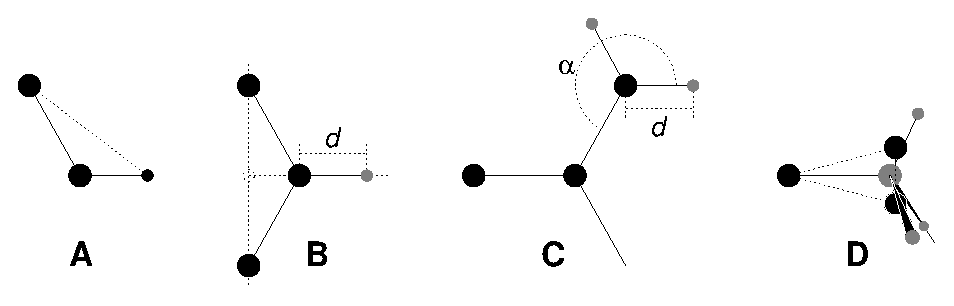
\includegraphics[width=11cm]{plots/dumtypes}}
\caption[Virtual site constructions for hydrogen atoms.]{The different
types of virtual site constructions used for hydrogen atoms. The atoms
used in the construction of the virtual site(s) are depicted as black
circles, virtual sites as gray ones. Hydrogens are smaller than heavy
atoms. {\sf A}: fixed bond angle, note that here the hydrogen is not a
virtual site; {\sf B}: in the plane of three atoms, with fixed distance;
{\sf C}: in the plane of three atoms, with fixed angle and distance;
{\sf D}: construction for amine groups ({\amine} or {\aminep}), see
text for details.}
\label{fig:vsitehydro}
\end{figure}

The goal of defining hydrogen atoms as virtual sites is to remove all
high-frequency degrees of freedom from them. In some cases, not all
degrees of freedom of a hydrogen atom should be removed, {\eg} in the
case of hydroxyl or amine groups the rotational freedom of the
hydrogen atom(s) should be preserved. Care should be taken that no
unwanted correlations are introduced by the construction of virtual
sites, {\eg} bond-angle vibration between the constructing atoms could
translate into hydrogen bond-length vibration. Additionally, since
virtual sites are by definition massless, in order to preserve total
system mass, the mass of each hydrogen atom that is treated as virtual
site should be added to the bonded heavy atom.

Taking into account these considerations, the hydrogen atoms in a
protein naturally fall into several categories, each requiring a
different approach (see also \figref{vsitehydro}).

\begin{itemize}

\item{\em hydroxyl ({\sf -OH}) or sulfhydryl ({\sf -SH})
hydrogen:\/} The only internal degree of freedom in a hydroxyl group
that can be constrained is the bending of the {\sf C-O-H} angle. This
angle is fixed by defining an additional bond of appropriate length,
see \figref{vsitehydro}A. Doing so removes the high-frequency angle bending,
but leaves the dihedral rotational freedom. The same goes for a
sulfhydryl group. {\bf Note} that in these cases the hydrogen is not treated
as a virtual site.

\item{\em single amine or amide ({\amines}) and aromatic hydrogens
({\sf -CH-}):\/} The position of these hydrogens cannot be constructed
from a linear combination of bond vectors, because of the flexibility
of the angle between the heavy atoms. Instead, the hydrogen atom is
positioned at a fixed distance from the bonded heavy atom on a line
going through the bonded heavy atom and a point on the line through
both second bonded atoms, see \figref{vsitehydro}B.

\item{\em planar amine ({\amine}) hydrogens:\/} The method used for
the single amide hydrogen is not well suited for planar amine groups,
because no suitable two heavy atoms can be found to define the
direction of the hydrogen atoms. Instead, the hydrogen is constructed
at a fixed distance from the nitrogen atom, with a fixed angle to the
carbon atom, in the plane defined by one of the other heavy atoms, see
\figref{vsitehydro}C.

\item{\em amine group (umbrella {\amine} or {\aminep}) hydrogens:\/}
Amine hydrogens with rotational freedom cannot be constructed as virtual
sites from the heavy atoms they are connected to, since this would
result in loss of the rotational freedom of the amine group. To
preserve the rotational freedom while removing the hydrogen bond-angle
degrees of freedom, two ``dummy masses'' are constructed with the same
total mass, moment of inertia (for rotation around the {\sf C-N} bond)
and center of mass as the amine group. These dummy masses have no
interaction with any other atom, except for the fact that they are
connected to the carbon and to each other, resulting in a rigid
triangle. From these three particles, the positions of the nitrogen and
hydrogen atoms are constructed as linear combinations of the two
carbon-mass vectors and their outer product, resulting in an amine
group with rotational freedom intact, but without other internal
degrees of freedom. See \figref{vsitehydro}D.

\end{itemize}

\begin{figure}
\centerline{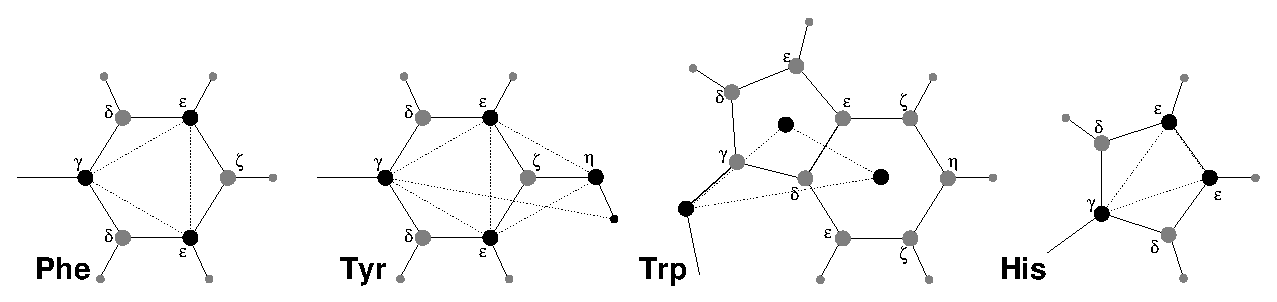
\includegraphics[width=15cm]{plots/dumaro}}
\caption[Virtual site constructions for aromatic residues.]{The
different types of virtual site constructions used for aromatic
residues. The atoms used in the construction of the virtual site(s) are
depicted as black circles, virtual sites as gray ones. Hydrogens are
smaller than heavy atoms. {\sf A}: phenylalanine; {\sf B}: tyrosine
(note that the hydroxyl hydrogen is {\em not} a virtual site); {\sf C}:
tryptophan; {\sf D}: histidine.}
\label{fig:vistearo}
\end{figure}

\subsection{Out-of-plane vibrations in aromatic groups}
\label{sec:vsitearo}
The planar arrangements in the side chains of the aromatic residues
lends itself perfectly to a virtual-site construction, giving a
perfectly planar group without the inherently unstable constraints
that are necessary to keep normal atoms in a plane. The basic approach
is to define three atoms or dummy masses with constraints between them
to fix the geometry and create the rest of the atoms as simple virtual
sites type (see \secref{virtual_sites}) from these three. Each of
the aromatic residues require a different approach:

\begin{itemize}

\item{\em Phenylalanine:\/} {\sf C}$_\gamma$, {\sf C}$_{{\epsilon}1}$,
and {\sf C}$_{{\epsilon}2}$ are kept as normal atoms, but with each a
mass of one third the total mass of the phenyl group. See
\figref{vsitehydro}A.

\item{\em Tyrosine:\/} The ring is treated identically to the
phenylalanine ring. Additionally, constraints are defined between {\sf
C}$_{{\epsilon}1}$, {\sf C}$_{{\epsilon}2}$, and {\sf O}$_{\eta}$.
The original improper dihedral angles will keep both triangles (one
for the ring and one with {\sf O}$_{\eta}$) in a plane, but due to the
larger moments of inertia this construction will be much more
stable. The bond-angle in the hydroxyl group will be constrained by a
constraint between {\sf C}$_\gamma$ and {\sf H}$_{\eta}$. {\bf Note} that
the hydrogen is not treated as a virtual site. See
\figref{vsitehydro}B.

\item{\em Tryptophan:\/} {\sf C}$_\beta$ is kept as a normal atom
and two dummy masses are created at the center of mass of each of the
rings, each with a mass equal to the total mass of the respective ring
({\sf C}$_{{\delta}2}$ and {\sf C}$_{{\epsilon}2}$ are each
counted half for each ring). This keeps the overall center of mass and
the moment of inertia almost (but not quite) equal to what it was. See
\figref{vsitehydro}C.

\item{\em Histidine:\/} {\sf C}$_\gamma$, {\sf C}$_{{\epsilon}1}$
and {\sf N}$_{{\epsilon}2}$ are kept as normal atoms, but with masses
redistributed such that the center of mass of the ring is
preserved. See \figref{vsitehydro}D.

\end{itemize}

\section{Viscosity calculation\index{viscosity}}

The shear viscosity is a property of liquids that can be determined easily  
by experiment. It is useful for parameterizing a force field
because it is a kinetic property, while most other properties
which are used for parameterization are thermodynamic.
The viscosity is also an important property, since it influences
the rates of conformational changes of molecules solvated in the liquid.

The viscosity can be calculated from an equilibrium simulation using
an Einstein relation:
\beq
\eta = \frac{1}{2}\frac{V}{k_B T} \lim_{t \rightarrow \infty}
\frac{\mbox{d}}{\mbox{d} t} \left\langle 
\left( \int_{t_0}^{{t_0}+t} P_{xz}(t') \mbox{d} t' \right)^2
\right\rangle_{t_0}
\eeq
This can be done with {\tt g_energy}.
This method converges very slowly~\cite{Hess2002a}, and as such
a nanosecond simulation might not
be long enough for an accurate determination of the viscosity.
The result is very dependent on the treatment of the electrostatics.
Using a (short) cut-off results in large noise on the off-diagonal
pressure elements, which can increase the calculated viscosity by an order
of magnitude.

{\gromacs} also has a non-equilibrium method for determining
the viscosity~\cite{Hess2002a}.
This makes use of the fact that energy, which is fed into system by
external forces, is dissipated through viscous friction. The generated heat
is removed by coupling to a heat bath. For a Newtonian liquid adding a 
small force will result in a velocity gradient according to the following
equation:
\beq
a_x(z) + \frac{\eta}{\rho} \frac{\partial^2 v_x(z)}{\partial z^2} = 0
\eeq
Here we have applied an acceleration $a_x(z)$ in the $x$-direction, which
is a function of the $z$-coordinate.
In {\gromacs} the acceleration profile is:
\beq
a_x(z) = A \cos\left(\frac{2\pi z}{l_z}\right)
\eeq
where $l_z$ is the height of the box. The generated velocity profile is:
\beq
v_x(z) = V \cos\left(\frac{2\pi z}{l_z}\right)
\eeq
\beq
V = A \frac{\rho}{\eta}\left(\frac{l_z}{2\pi}\right)^2
\eeq
The viscosity can be calculated from $A$ and $V$:
\beq
\label{visc}
\eta = \frac{A}{V}\rho \left(\frac{l_z}{2\pi}\right)^2
\eeq

In the simulation $V$ is defined as:
\beq
V = \frac{\displaystyle \sum_{i=1}^N m_i v_{i,x} 2 \cos\left(\frac{2\pi z}{l_z}\right)}
         {\displaystyle \sum_{i=1}^N m_i}
\eeq
The generated velocity profile is not coupled to the heat bath. Moreover,
the velocity profile is excluded from the kinetic energy.
One would like $V$ to be as large as possible to get good statistics.
However, the shear rate should not be so high that the system gets too far
from equilibrium. The maximum shear rate occurs where the cosine is zero,
the rate being:
\beq
\mbox{sh}_{\max} =  \max_z \left| \frac{\partial v_x(z)}{\partial z} \right|
= A \frac{\rho}{\eta} \frac{l_z}{2\pi}
\eeq
For a simulation with: $\eta=10^{-3}$ [kg\,m$^{-1}$\,s$^{-1}$],
$\rho=10^3$\,[kg\,m$^{-3}$] and $l_z=2\pi$\,[nm],
$\mbox{sh}_{\max}=1$\,[ps\,nm$^{-1}$] $A$.
This shear rate should be smaller than one over the longest
correlation time in the system. For most liquids, this will be the rotation
correlation time, which is around 10 ps. In this case, $A$ should
be smaller than 0.1\,[nm\,ps$^{-2}$].
When the shear rate is too high, the observed viscosity will be too low.
Because $V$ is proportional to the square of the box height,
the optimal box is elongated in the $z$-direction.
In general, a simulation length of 100 ps is enough to obtain an
accurate value for the viscosity.

The heat generated by the viscous friction is removed by coupling to a heat
bath. Because this coupling is not instantaneous the real temperature of the
liquid will be slightly lower than the observed temperature.
Berendsen derived this temperature shift~\cite{Berendsen91}, which can
be written in terms of the shear rate as:
\beq
T_s = \frac{\eta\,\tau}{2 \rho\,C_v} \mbox{sh}_{\max}^2
\eeq
where $\tau$ is the coupling time for the Berendsen thermostat and
$C_v$ is the heat capacity. Using the values of the example above,
$\tau=10^{-13}$ [s] and $C_v=2 \cdot 10^3$\,[J kg$^{-1}$\,K$^{-1}$], we
get: $T_s=25$\,[K\,ps$^{-2}$]\,sh$_{\max}^2$. When we want the shear
rate to be smaller than $1/10$\,[ps$^{-1}$], $T_s$ is smaller than
0.25\,[K], which is negligible.

{\bf Note} that the system has to build up the velocity profile when starting
from an equilibrium state. This build-up time is of the order of the
correlation time of the liquid.

Two quantities are written to the energy file, along with their averages
and fluctuations: $V$ and $1/\eta$, as obtained from (\ref{visc}).

\section{Tabulated interaction functions\index{tabulated interaction functions}}
\subsection{Cubic splines for potentials}
\label{subsec:cubicspline}
In some of the inner loops of {\gromacs}, look-up tables are used 
for computation of potential and forces. 
The tables are interpolated using a cubic
spline algorithm. 
There are separate tables for electrostatic, dispersion, and repulsion
interactions,
but for the sake of caching performance these have been combined
into a single array. 
The cubic spline interpolation for $x_i \leq x < x_{i+1}$ looks like this:
\beq
V_s(x) = A_0 + A_1 \,\epsilon + A_2 \,\epsilon^2 + A_3 \,\epsilon^3
\label{eqn:spline}
\eeq
where the table spacing $h$ and fraction $\epsilon$ are given by:
\bea
h	&=&	x_{i+1} - x_i	\\
\epsilon&=&	(x - x_i)/h
\eea
so that $0 \le \epsilon < 1$.
From this, we can calculate the derivative in order to determine the forces:
\beq
-V_s'(x) ~=~ 
-\frac{{\rm d}V_s(x)}{{\rm d}\epsilon}\frac{{\rm d}\epsilon}{{\rm d}x} ~=~
-(A_1 + 2 A_2 \,\epsilon + 3 A_3 \,\epsilon^2)/h
\eeq
The four coefficients are determined from the four conditions
that $V_s$ and $-V_s'$ at both ends of each interval should match
the exact potential $V$ and force $-V'$.
This results in the following errors for each interval:
\bea
|V_s  - V  |_{max} &=& V'''' \frac{h^4}{384} + O(h^5) \\
|V_s' - V' |_{max} &=& V'''' \frac{h^3}{72\sqrt{3}} + O(h^4) \\
|V_s''- V''|_{max} &=& V'''' \frac{h^2}{12}  + O(h^3)
\eea
V and V' are continuous, while V'' is the first discontinuous
derivative.
The number of points per nanometer is 500 and 2000
for mixed- and double-precision versions of {\gromacs}, respectively.
This means that the errors in the potential and force will usually
be smaller than the mixed precision accuracy.

{\gromacs} stores $A_0$, $A_1$, $A_2$ and $A_3$.
The force routines get a table with these four parameters and
a scaling factor $s$ that is equal to the number of points per nm.
({\bf Note} that $h$ is $s^{-1}$).
The algorithm goes a little something like this:
\begin{enumerate}
\item	Calculate distance vector (\ve{r}$_{ij}$) and distance r$_{ij}$
\item	Multiply r$_{ij}$ by $s$ and truncate to an integer value $n_0$
	to get a table index
\item	Calculate fractional component ($\epsilon$ = $s$r$_{ij} - n_0$) 
	and $\epsilon^2$ 
\item	Do the interpolation to calculate the potential $V$ and the scalar force $f$
\item	Calculate the vector force \ve{F} by multiplying $f$ with \ve{r}$_{ij}$
\end{enumerate}

{\bf Note} that table look-up is significantly {\em
slower} than computation of the most simple Lennard-Jones and Coulomb
interaction. However, it is much faster than the shifted Coulomb
function used in conjunction with the PPPM method. Finally, it is much
easier to modify a table for the potential (and get a graphical
representation of it) than to modify the inner loops of the MD
program.

\subsection{User-specified potential functions}
\label{subsec:userpot}
You can also use your own potential functions\index{potential function} without 
editing the {\gromacs} code.  The potential function should be according to the 
following equation
\beq
V(r_{ij}) ~=~ \frac{q_i q_j}{4 \pi\epsilon_0} f(r_{ij}) + C_6 \,g(r_{ij}) + C_{12} \,h(r_{ij})
\eeq
where $f$, $g$, and $h$ are user defined functions. {\bf Note} that if $g(r)$ represents a
normal dispersion interaction, $g(r)$ should be $<$ 0. C$_6$, C$_{12}$
and the charges are read from the topology. Also note that combination
rules are only supported for Lennard-Jones and Buckingham, and that
your tables should match the parameters in the binary topology.

When you add the following lines in your {\tt .mdp} file:

{\small
\begin{verbatim}
rlist           = 1.0
coulombtype     = User
rcoulomb        = 1.0
vdwtype         = User
rvdw            = 1.0
\end{verbatim}}

{\tt mdrun} will read a single non-bonded table file,
or multiple when {\tt energygrp-table} is set (see below).
The name of the file(s) can be set with the {\tt mdrun} option {\tt -table}.
The table file should contain seven columns of table look-up data in the
order: $x$, $f(x)$, $-f'(x)$, $g(x)$, $-g'(x)$, $h(x)$, $-h'(x)$.
The $x$ should run from 0 to $r_c+1$ (the value of {\tt table_extension} can be
changed in the {\tt .mdp} file).
You can choose the spacing you like; for the standard tables {\gromacs}
uses a spacing of 0.002 and 0.0005 nm when you run in mixed
and double precision, respectively.  In this
context, $r_c$ denotes the maximum of the two cut-offs {\tt rvdw} and
{\tt rcoulomb} (see above). These variables need not be the same (and
need not be 1.0 either).  Some functions used for potentials contain a
singularity at $x = 0$, but since atoms are normally not closer to each
other than 0.1 nm, the function value at $x = 0$ is not important.
Finally, it is also
possible to combine a standard Coulomb with a modified LJ potential
(or vice versa). One then specifies {\eg} {\tt coulombtype = Cut-off} or
{\tt coulombtype = PME}, combined with {\tt vdwtype = User}.  The table file must
always contain the 7 columns however, and meaningful data (i.e. not
zeroes) must be entered in all columns.  A number of pre-built table
files can be found in the {\tt GMXLIB} directory for 6-8, 6-9, 6-10, 6-11, and 6-12
Lennard-Jones potentials combined with a normal Coulomb.

If you want to have different functional forms between different
groups of atoms, this can be set through energy groups.
Different tables can be used for non-bonded interactions between
different energy groups pairs through the {\tt .mdp} option {\tt energygrp-table}
(see details in the User Guide).
Atoms that should interact with a different potential should
be put into different energy groups.
Between group pairs which are not listed in {\tt energygrp-table},
the normal user tables will be used. This makes it easy to use
a different functional form between a few types of atoms.

\section{Mixed Quantum-Classical simulation techniques}

In a molecular mechanics (MM) force field, the influence of electrons
is expressed by empirical parameters that are assigned on the basis of
experimental data, or on the basis of results from high-level quantum
chemistry calculations. These are valid for the ground state of a
given covalent structure, and the MM approximation is usually
sufficiently accurate for ground-state processes in which the overall
connectivity between the atoms in the system remains
unchanged. However, for processes in which the connectivity does
change, such as chemical reactions, or processes that involve multiple
electronic states, such as photochemical conversions, electrons can no
longer be ignored, and a quantum mechanical description is required
for at least those parts of the system in which the reaction takes
place.

One approach to the simulation of chemical reactions in solution, or
in enzymes, is to use a combination of quantum mechanics (QM) and
molecular mechanics (MM). The reacting parts of the system are treated
quantum mechanically, with the remainder being modeled using the
force field. The current version of {\gromacs} provides interfaces to
several popular Quantum Chemistry packages (MOPAC~\cite{mopac},
GAMESS-UK~\cite{gamess-uk}, Gaussian~\cite{g03} and CPMD~\cite{Car85a}).

{\gromacs} interactions between the two subsystems are
either handled as described by Field {\em et al.}~\cite{Field90a} or
within the ONIOM approach by Morokuma and coworkers~\cite{Maseras96a,
Svensson96a}.

\subsection{Overview}

Two approaches for describing the interactions between the QM and MM
subsystems are supported in this version:

\begin{enumerate}
\item{\textbf{Electronic Embedding}} The electrostatic interactions
between the electrons of the QM region and the MM atoms and between
the QM nuclei and the MM atoms are included in the Hamiltonian for
the QM subsystem: \beq H^{QM/MM} =
H^{QM}_e-\sum_i^n\sum_J^M\frac{e^2Q_J}{4\pi\epsilon_0r_{iJ}}+\sum_A^N\sum_J^M\frac{e^2Z_AQ_J}{e\pi\epsilon_0R_{AJ}},
\eeq where $n$ and $N$ are the number of electrons and nuclei in the
QM region, respectively, and $M$ is the number of charged MM
atoms. The first term on the right hand side is the original
electronic Hamiltonian of an isolated QM system. The first of the
double sums is the total electrostatic interaction between the QM
electrons and the MM atoms. The total electrostatic interaction of the
QM nuclei with the MM atoms is given by the second double sum. Bonded
interactions between QM and MM atoms are described at the MM level by
the appropriate force-field terms. Chemical bonds that connect the two
subsystems are capped by a hydrogen atom to complete the valence of
the QM region. The force on this atom, which is present in the QM
region only, is distributed over the two atoms of the bond. The cap
atom is usually referred to as a link atom.

\item{\textbf{ONIOM}} In the ONIOM approach, the energy and gradients
are first evaluated for the isolated QM subsystem at the desired level
of {\it{ab initio}} theory. Subsequently, the energy and gradients of
the total system, including the QM region, are computed using the
molecular mechanics force field and added to the energy and gradients
calculated for the isolated QM subsystem. Finally, in order to correct
for counting the interactions inside the QM region twice, a molecular
mechanics calculation is performed on the isolated QM subsystem and
the energy and gradients are subtracted. This leads to the following
expression for the total QM/MM energy (and gradients likewise): \beq
E_{tot} = E_{I}^{QM}
+E_{I+II}^{MM}-E_{I}^{MM}, \eeq where the
subscripts I and II refer to the QM and MM subsystems,
respectively. The superscripts indicate at what level of theory the
energies are computed. The ONIOM scheme has the
advantage that it is not restricted to a two-layer QM/MM description,
but can easily handle more than two layers, with each layer described
at a different level of theory.
\end{enumerate}

\subsection{Usage}

To make use of the QM/MM functionality in {\gromacs}, one needs to:

\begin{enumerate}
\item introduce link atoms at the QM/MM boundary, if needed;
\item specify which atoms are to be treated at a QM level;
\item specify the QM level, basis set, type of QM/MM interface and so on. 
\end{enumerate}

\subsubsection{Adding link atoms}

At the bond that connects the QM and MM subsystems, a link atoms is
introduced.  In {\gromacs} the link atom has special atomtype, called
LA. This atomtype is treated as a hydrogen atom in the QM calculation,
and as a virtual site in the force-field calculation. The link atoms, if
any, are part of the system, but have no interaction with any other
atom, except that the QM force working on it is distributed over the
two atoms of the bond. In the topology, the link atom (LA), therefore,
is defined as a virtual site atom:

{\small
\begin{verbatim}
[ virtual_sites2 ]
LA QMatom MMatom 1 0.65
\end{verbatim}}

See~\secref{vsitetop} for more details on how virtual sites are
treated. The link atom is replaced at every step of the simulation.

In addition, the bond itself is replaced by a constraint:

{\small
\begin{verbatim}
[ constraints ]
QMatom MMatom 2 0.153
\end{verbatim}}

{\bf Note} that, because in our system the QM/MM bond is a carbon-carbon
bond (0.153 nm), we use a constraint length of 0.153 nm, and dummy
position of 0.65. The latter is the ratio between the ideal C-H
bond length and the ideal C-C bond length. With this ratio, the link
atom is always 0.1 nm away from the {\tt QMatom}, consistent with the
carbon-hydrogen bond length. If the QM and MM subsystems are connected
by a different kind of bond, a different constraint and a different
dummy position, appropriate for that bond type, are required.

\subsubsection{Specifying the QM atoms}

Atoms that should be treated at a QM level of theory, including the
link atoms, are added to the index file. In addition, the chemical
bonds between the atoms in the QM region are to be defined as
connect bonds (bond type 5) in the topology file:

{\small
\begin{verbatim}
[ bonds ]
QMatom1 QMatom2 5
QMatom2 QMatom3 5
\end{verbatim}}

\subsubsection{Specifying the QM/MM simulation parameters}

In the {\tt .mdp} file, the following parameters control a QM/MM simulation.

\begin{description}

\item[\tt QMMM = no]\mbox{}\\ If this is set to {\tt yes}, a QM/MM
simulation is requested. Several groups of atoms can be described at
different QM levels separately. These are specified in the QMMM-grps
field separated by spaces. The level of {\it{ab initio}} theory at which the
groups are described is specified by {\tt QMmethod} and {\tt QMbasis}
Fields. Describing the groups at different levels of theory is only
possible with the ONIOM QM/MM scheme, specified by {\tt QMMMscheme}.

\item[\tt QMMM-grps =]\mbox{}\\groups to be described at the QM level

\item[\tt QMMMscheme = normal]\mbox{}\\Options are {\tt normal} and
{\tt ONIOM}. This selects the QM/MM interface. {\tt normal} implies
that the QM subsystem is electronically embedded in the MM
subsystem. There can only be one {\tt QMMM-grps} that is modeled at
the {\tt QMmethod} and {\tt QMbasis} level of {\it{ ab initio}}
theory. The rest of the system is described at the MM level. The QM
and MM subsystems interact as follows: MM point charges are included
in the QM one-electron Hamiltonian and all Lennard-Jones interactions
are described at the MM level. If {\tt ONIOM} is selected, the
interaction between the subsystem is described using the ONIOM method
by Morokuma and co-workers. There can be more than one QMMM-grps each
modeled at a different level of QM theory (QMmethod and QMbasis).

\item[\tt QMmethod = ]\mbox{}\\Method used to compute the energy
and gradients on the QM atoms. Available methods are AM1, PM3, RHF,
UHF, DFT, B3LYP, MP2, CASSCF, MMVB and CPMD. For CASSCF, the number of
electrons and orbitals included in the active space is specified by
{\tt CASelectrons} and {\tt CASorbitals}. For CPMD, the plane-wave
cut-off is specified by the {\tt planewavecutoff} keyword.

\item[\tt QMbasis = ]\mbox{}\\Gaussian basis set used to expand the
electronic wave-function. Only Gaussian basis sets are currently
available, i.e. STO-3G, 3-21G, 3-21G*, 3-21+G*, 6-21G, 6-31G, 6-31G*,
6-31+G*, and 6-311G. For CPMD, which uses plane wave expansion rather
than atom-centered basis functions, the {\tt planewavecutoff} keyword
controls the plane wave expansion.

\item[\tt QMcharge = ]\mbox{}\\The total charge in {\it{e}} of the {\tt
QMMM-grps}. In case there are more than one {\tt QMMM-grps}, the total
charge of each ONIOM layer needs to be specified separately.

\item[\tt QMmult = ]\mbox{}\\The multiplicity of the {\tt
QMMM-grps}. In case there are more than one {\tt QMMM-grps}, the
multiplicity of each ONIOM layer needs to be specified separately.

\item[\tt CASorbitals = ]\mbox{}\\The number of orbitals to be
included in the active space when doing a CASSCF computation.

\item[\tt CASelectrons = ]\mbox{}\\The number of electrons to be
included in the active space when doing a CASSCF computation.

\item[\tt SH = no]\mbox{}\\If this is set to yes, a QM/MM MD
simulation on the excited state-potential energy surface and enforce a
diabatic hop to the ground-state when the system hits the conical
intersection hyperline in the course the simulation. This option only
works in combination with the CASSCF method.

\end{description}

\subsection{Output}

The energies and gradients computed in the QM calculation are added to
those computed by {\gromacs}. In the {\tt .edr} file there is a section
for the total QM energy.

\subsection{Future developments}

Several features are currently under development to increase the
accuracy of the QM/MM interface. One useful feature is the use of
delocalized MM charges in the QM computations. The most important
benefit of using such smeared-out charges is that the Coulombic
potential has a finite value at interatomic distances. In the point
charge representation, the partially-charged MM atoms close to the QM
region tend to ``over-polarize'' the QM system, which leads to artifacts
in the calculation.

What is needed as well is a transition state optimizer.

\section{Using VMD plug-ins for trajectory file I/O}
\index{VMD plug-ins}\index{trajectory file}{\gromacs} tools are able
to use the plug-ins found in an existing installation of
\href{http://www.ks.uiuc.edu/Research/vmd}{VMD} in order to read and
write trajectory files in formats that are not native to
{\gromacs}. You will be able to supply an AMBER DCD-format trajectory
filename directly to {\gromacs} tools, for example.

This requires a VMD installation not older than version 1.8, that your
system provides the dlopen function so that programs can determine at
run time what plug-ins exist, and that you build shared libraries when
building {\gromacs}. CMake will find the vmd executable in your path, and
from it, or the environment variable {\tt VMDDIR} at configuration or
run time, locate the plug-ins. Alternatively, the {\tt VMD_PLUGIN_PATH}
can be used at run time to specify a path where these plug-ins can be
found. Note that these plug-ins are in a binary format, and that format
must match the architecture of the machine attempting to use them.


\section{\normindex{Interactive Molecular Dynamics}}
{\gromacs} supports the interactive molecular dynamics (IMD) protocol as implemented
by \href{http://www.ks.uiuc.edu/Research/vmd}{VMD} to control a running simulation
in NAMD. IMD allows to monitor a running {\gromacs} simulation from a VMD client.
In addition, the user can interact with the simulation by pulling on atoms, residues
or fragments with a mouse or a force-feedback device. Additional information about
the {\gromacs} implementation and an exemplary {\gromacs} IMD system can be found
\href{http://www.mpibpc.mpg.de/grubmueller/interactivemd}{on this homepage}.

\subsection{Simulation input preparation}
The {\gromacs} implementation allows transmission and interaction with a part of the
running simulation only, e.g.\ in cases where no water molecules should be transmitted
or pulled. The group is specified via the {\tt .mdp} option {\tt IMD-group}. When
{\tt IMD-group} is empty, the IMD protocol is disabled and cannot be enabled via the
switches in {\tt mdrun}. To interact with the entire system, {\tt IMD-group} can
be set to {\tt System}. When using {\tt grompp}, a {\tt .gro} file
to be used as VMD input is written out ({\tt -imd} switch of {\tt grompp}).

\subsection{Starting the simulation}
Communication between VMD and {\gromacs} is achieved via TCP sockets and thus enables
controlling an {\tt mdrun} running locally or on a remote cluster. The port for the
connection can be specified with the {\tt -imdport} switch of {\tt mdrun}, 8888 is
the default. If a port number of 0 or smaller is provided, {\gromacs} automatically
assigns a free port to use with IMD.

Every $N$ steps, the {\tt mdrun} client receives the applied forces from VMD and sends the new
positions to the client. VMD permits increasing or decreasing the communication frequency
interactively.
By default, the simulation starts and runs even if no IMD client is connected. This
behavior is changed by the {\tt -imdwait} switch of {\tt mdrun}. After startup and
whenever the client has disconnected, the integration stops until reconnection of
the client.
When the {\tt -imdterm} switch is used, the simulation can be terminated by pressing
the stop button in VMD. This is disabled by default.
Finally, to allow interacting with the simulation (i.e. pulling from VMD) the {\tt -imdpull}
switch has to be used.
Therefore, a simulation can only be monitored but not influenced from the VMD client
when none of {\tt -imdwait}, {\tt -imdterm} or {\tt -imdpull} are set. However, since
the IMD protocol requires no authentication, it is not advisable to run simulations on
a host directly reachable from an insecure environment. Secure shell forwarding of TCP
can be used to connect to running simulations not directly reachable from the interacting host.
Note that the IMD command line switches of {\tt mdrun} are hidden by default and show
up in the help text only with {\tt gmx mdrun -h -hidden}.

\subsection{Connecting from VMD}
In VMD, first the structure corresponding to the IMD group has to be loaded ({\it File
$\rightarrow$ New Molecule}). Then the IMD connection window has to be used
({\it Extensions $\rightarrow$ Simulation $\rightarrow$ IMD Connect (NAMD)}). In the IMD
connection window, hostname and port have to be specified and followed by pressing
{\it Connect}. {\it Detach Sim} allows disconnecting without terminating the simulation, while
{\it Stop Sim} ends the simulation on the next neighbor searching step (if allowed by
{\tt -imdterm}).

The timestep transfer rate allows adjusting the communication frequency between simulation
and IMD client. Setting the keep rate loads every $N^\mathrm{th}$ frame into VMD instead
of discarding them when a new one is received. The displayed energies are in SI units
in contrast to energies displayed from NAMD simulations.

\section{\normindex{Embedding proteins into the membranes}}
\label{sec:membed}

GROMACS is capable of inserting the protein into pre-equilibrated
lipid bilayers with minimal perturbation of the lipids using the
method, which was initially described as a ProtSqueeze
technique,\cite{Yesylevskyy2007} and later implemented as g\_membed
tool.\cite{Wolf2010} Currently the functionality of g\_membed is
available in mdrun as described in the user guide.

This method works by first artificially shrinking the protein in the
$xy$-plane, then it removes lipids that overlap with that much smaller
core. Then the protein atoms are gradually resized back to their
initial configuration, using normal dynamics for the rest of the
system, so the lipids adapt to the protein. Further lipids are removed
as required.


% LocalWords:  PMF pmf kJ mol Jarzynski BT bilayer rup mdp AFM fepmf fecalc rb
% LocalWords:  posre grompp fs Verlet dihedrals hydrogens hydroxyl sulfhydryl
% LocalWords:  vsitehydro planarity chirality pdb gmx virtualize virtualized xz
% LocalWords:  vis massless tryptophan histidine phenyl parameterizing ij PPPM
% LocalWords:  parameterization Berendsen rlist coulombtype rcoulomb vdwtype LJ
% LocalWords:  rvdw energygrp mdrun pre GMXLIB MOPAC GAMESS CPMD ONIOM
% LocalWords:  Morokuma iJ AQ AJ initio atomtype QMatom MMatom QMMM grps et al
% LocalWords:  QMmethod QMbasis QMMMscheme RHF DFT LYP CASSCF MMVB CASelectrons
% LocalWords:  CASorbitals planewavecutoff STO QMcharge QMmult diabatic edr
% LocalWords:  hyperline delocalized Coulombic indices nm ccc th ps
% LocalWords:  GTX CPUs GHz md sd bd vv avek tcoupl andersen tc OPLSAA GROMOS
% LocalWords:  OBC obc CCMA tol pbc xyz barostat pcoupl acc gpu PLUGIN Cmake GX
% LocalWords:  MSVC gcc installpath cmake DGMX DCMAKE functionalities GPGPU GTS
% LocalWords:  OpenCL DeviceID gromacs gpus html GeForce Quadro FX Plex CX GF
% LocalWords:  VMD DCD GROningen MAchine BIOSON Groningen der Spoel Drunen Comp
% LocalWords:  Phys Comm moltype intramol vdw Waals fep multivector pf
% LocalWords:  pymbar dhdl xvg LINCS Entropic entropic solutes ref com iso pm
% LocalWords:  rm prefactors equipotential potiso potisopf potpm trr
% LocalWords:  potrm potrmpf midplanes midplane gaussians potflex vars massw av
% LocalWords:  shure observables rccccccc vec eps dist min eqn transl nstsout
% LocalWords:  nstrout rotangles rotslabs rottorque RMSD rmsdfit excl NH amine
% LocalWords:  positionrestraint es SH phenylalanine solvated sh nanometer QM
% LocalWords:  Lennard Buckingham UK Svensson ab vsitetop co UHF MP interatomic
% LocalWords:  cg grp coords SPC userpot
% LocalWords:  itp sitesn atomtypes ff csg ndx Tesla CHARMM AA gauss
% LocalWords:  CMAP nocmap fators Monte performant lib LD DIR llllcc
% LocalWords:  CMake homepage DEV overclocking GT dlopen vmd VMDDIR
% LocalWords:  versa PME atomperatom graining forcefields hy spc OPLS
% LocalWords:  topol multi
